\documentclass[11pt,letterpaper]{article}
\usepackage{fontspec}
\setmainfont{texgyrepagella}[Extension=.otf,UprightFont=*-regular,BoldFont=*-bold,ItalicFont=*-italic,BoldItalicFont=*-bolditalic]
\usepackage[bidi=default]{babel}
\babelprovide[import,main]{spanish}
\babelprovide[import]{hebrew}
\babelprovide[import]{ancientgreek}
\babelfont[hebrew]{rm}[Path=fonts/,BoldFont=NotoHebrewSerif-700.ttf,Scale=0.95]{NotoHebrewSerif-400.ttf}
\babelfont[ancientgreek]{rm}[Path=fonts/]{GFSPorson.otf}
\newcommand{\heb}[1]{\mbox{\foreignlanguage{hebrew}{#1}}}
\newcommand{\grc}[1]{\foreignlanguage{ancientgreek}{#1}}
\newcommand{\hebverso}[1]{\par\smallskip{\centering\begin{otherlanguage}{hebrew}\large #1\end{otherlanguage}\par}\smallskip}
\newcommand{\SENOR}{\textsc{Señor}}
\usepackage[margin=2.5cm,headheight=14pt]{geometry}
\usepackage{microtype,ragged2e,booktabs,graphicx,xcolor,csquotes,array}
\usepackage[hidelinks]{hyperref}\usepackage{xurl}\urlstyle{same}
\usepackage[most]{tcolorbox}
\usepackage{tikz}\usetikzlibrary{arrows.meta,positioning,calc,decorations.pathreplacing,shapes.geometric}
\usepackage{titlesec,fancyhdr}
\definecolor{tierraroja}{RGB}{122,40,18}\definecolor{caferojizo}{RGB}{58,18,8}
\definecolor{mostaza}{RGB}{214,160,58}\definecolor{papiro}{RGB}{243,228,192}\definecolor{sepia}{RGB}{98,66,44}
\definecolor{oliva}{RGB}{92,98,48}
\titleformat{\section}{\Large\bfseries\color{tierraroja}}{\thesection.}{0.6em}{}
\titleformat{\subsection}{\large\bfseries\color{caferojizo}}{\thesubsection}{0.6em}{}
\pagestyle{fancy}\fancyhf{}
\fancyhead[L]{\foreignlanguage{spanish}{\small\itshape\color{sepia}El Jubileo}}\fancyhead[R]{\foreignlanguage{spanish}{\small\color{sepia}\thepage}}
\renewcommand{\headrulewidth}{0.4pt}
\setlength{\parindent}{1.27cm}\linespread{1.15}\setlength{\emergencystretch}{3em}
\newtcolorbox{cita}[1][]{enhanced,unbreakable,colback=tierraroja!5!white,colframe=tierraroja,boxrule=0pt,leftrule=2.5pt,arc=0pt,
  left=8pt,right=8pt,top=5pt,bottom=5pt,before skip=8pt,after skip=8pt,fontupper=\itshape,#1}
\newcommand{\fuente}[1]{\par\hfill{\upshape\bfseries\small\textcolor{tierraroja}{#1}}}
\newtcolorbox{nota}[1][]{enhanced,unbreakable,colback=mostaza!10,colframe=mostaza!85!tierraroja,boxrule=0.6pt,arc=2pt,
  fonttitle=\bfseries\small,coltitle=caferojizo,colbacktitle=mostaza!30,fontupper=\small,title={#1}}
\newtcolorbox{filologia}[1][]{enhanced,unbreakable,colback=white,colframe=tierraroja!45,boxrule=0.5pt,arc=2pt,
  fonttitle=\bfseries\small,coltitle=white,colbacktitle=tierraroja!80,fontupper=\small,title={Filología: #1}}
\newcommand{\refapa}[1]{\par{\RaggedRight\hangindent=1.27cm\hangafter=1\noindent #1\par}\vspace{4pt}}
\newcommand{\destacar}[1]{\textbf{\textcolor{tierraroja}{#1}}}
\newcolumntype{L}[1]{>{\RaggedRight\arraybackslash}p{#1}}
\newcommand{\pie}[1]{\par{\footnotesize\color{sepia}#1\par}}

\title{\color{tierraroja}\bfseries El Jubileo: proclamaréis libertad en la tierra\\[4pt]\large\color{sepia}\mdseries ``Pregonaréis libertad en la tierra a todos sus moradores'' (Lv 25:10)}
\author{}\date{}
\begin{document}
\maketitle\thispagestyle{empty}

\begin{abstract}\noindent
Cada cuarenta y nueve años, el día diez del mes séptimo, en el Día de la Expiación, el shofar de \emph{teruá} debía recorrer toda la tierra de Israel para anunciar el año cincuenta: \emph{derór}, liberación, para todos sus moradores; cada uno volvería a su posesión y a su familia (Lv 25:8--10). El Jubileo (\emph{yovel}) no figura entre las convocaciones de Levítico~23, pero se proclama dentro de una de ellas y lleva a su consecuencia social lo que el Día de la Expiación hace en el santuario: después del perdón, la libertad; después de la libertad, el retorno a la heredad. Este capítulo lee Levítico 25:8--55 y sus ecos (Lv 27; Nm 36; Rut 4; Jer 32 y 34; Ez 46; Is 49, 58 y 61) con el método de la serie. La lectura histórica sitúa la ley en el sistema israelita de tierra, clan y herencia y la compara con los edictos de remisión mesopotámicos (\emph{andurārum}, \emph{mīšarum}); discute si se practicó y sigue su relectura en el Libro de los Jubileos y en 11QMelquisedec. La lectura filológica estudia \emph{yovel}, \emph{derór}, \emph{ge'ulá} y \emph{goel}, \emph{ajuzá}, \emph{najalá}, \emph{tsemitut}, \emph{guer} y \emph{toshav}, y su paso al griego (\emph{áphesis}, \emph{lytrōsis}, \emph{apolytrōsis}, \emph{dektós}, \emph{apokatástasis}). La lectura textual examina cómo Lucas 4:18--19 une Isaías 61 con Isaías 58:6 y se detiene antes del ``día de venganza''. La lectura literaria muestra la cuenta 7\,×\,7\,+\,1 que comparte con Shavuot y la estructura de Levítico 25 en círculos de redención. La síntesis expone la lectura de la serie: el Jubileo como figura de la redención completa y del reposo que queda para el pueblo de Dios.
\par\smallskip\noindent\textbf{Palabras clave:} Jubileo, \emph{yovel}, \emph{derór}, \emph{goel}, redención, Levítico 25, Isaías 61, Lucas 4, \emph{áphesis}, Día de la Expiación.\end{abstract}

\begin{nota}[Nota sobre el texto]
Las citas bíblicas son de la Reina-Valera 1960 (RVR1960), convención de esta serie; donde esa versión escribe ``Jehová'' se escribe aquí \SENOR, que traduce el tetragrama \heb{יהוה}. Cuando la redacción exacta de la RVR1960 no es segura, se parafrasea sin comillas o se marca ``(trad. propia)''. El hebreo sigue la \emph{Biblia Hebraica Stuttgartensia}; el griego, el NA28 y la Septuaginta de Rahlfs-Hanhart. Las fuentes judías (Misná, Talmud, Sifra, Rashi) se citan desde Sefaria y se marcan como tradición posterior. Las lecturas tipológicas de la serie y los cálculos cronológicos se señalan como \emph{Precisión}. Los conteos de palabras son propios: se hicieron por lema (número de Strong) sobre el Códice de Leningrado etiquetado morfológicamente.
\end{nota}

%===================================================================
\section{Introducción: la trompeta que suena el día del perdón}

¿Por qué la libertad se anuncia el Día de la Expiación? La ley podría haber fijado el Jubileo en el primer día del año o en la alegría de Cabañas. Levítico 25:9 lo fija en el día más solemne del calendario, el único de ayuno, cuando el sumo sacerdote entraba en el Lugar Santísimo con la sangre del macho cabrío ``por Jehová'' (Lv 16:15--16). Ese día, en el año cincuenta, al terminar la expiación del santuario, el shofar debía sonar ``por toda vuestra tierra''. Primero Dios limpia al pueblo y después lo suelta; el orden importa, y buena parte de este estudio consiste en explicar por qué.

Mi lectura es que el Jubileo lleva al terreno social, económico y territorial lo que el Día de la Expiación realiza en el santuario. Se apoya en dos frases de Dios, ``la tierra mía es'' (Lv 25:23) y ``son mis siervos, los cuales saqué yo de la tierra de Egipto'' (Lv 25:42). Porque la tierra y el pueblo pertenecen a Dios, nadie puede quedarse para siempre con la heredad de otro ni con la vida de su hermano. La deuda, la pobreza y la servidumbre son reales, pero tienen fecha de término. Los profetas tomaron esa institución como imagen de la restauración final (Is 61:1--3), Jesús la leyó en la sinagoga de Nazaret como programa de su misión (Lc 4:18--21) y los apóstoles describieron la obra de Cristo con el vocabulario del rescate del pariente (\emph{goel}). Dentro de la serie, el Jubileo queda así como figura de la redención completa: expiación, libertad y retorno a la heredad.

El recorrido es el habitual. Primero el texto (Lv 25 y sus paralelos, en una tabla sinóptica); después cuatro lecturas: histórica (tierra, clan y herencia; los edictos de remisión del antiguo Cercano Oriente; si el Jubileo se practicó; su relectura en el Segundo Templo), filológica (\emph{yovel}, \emph{derór}, \emph{goel} y su paso al griego), textual (Lucas 4 frente a Isaías 61, el cómputo del año cincuenta) y literaria (la cuenta de cincuenta, la estructura de Levítico 25, el Jubileo en los profetas). Dos secciones siguen al pariente que rescata, en la ley, en Rut, en Jeremías y en Isaías, y al año de la redención de Isaías 63 y Abdías. Cierran la lectura de la serie, el Jubileo en Jesús y los apóstoles, la tradición judía, la discusión de interpretaciones y la síntesis.

El Jubileo no es una de las siete fiestas de Levítico 23, porque es un año y no un día; pero se anuncia dentro del ciclo, en el sexto de sus hitos:

\begin{center}\begin{minipage}{\linewidth}\centering
% === Esquema estándar de la serie: el ciclo de Levítico 23 ===
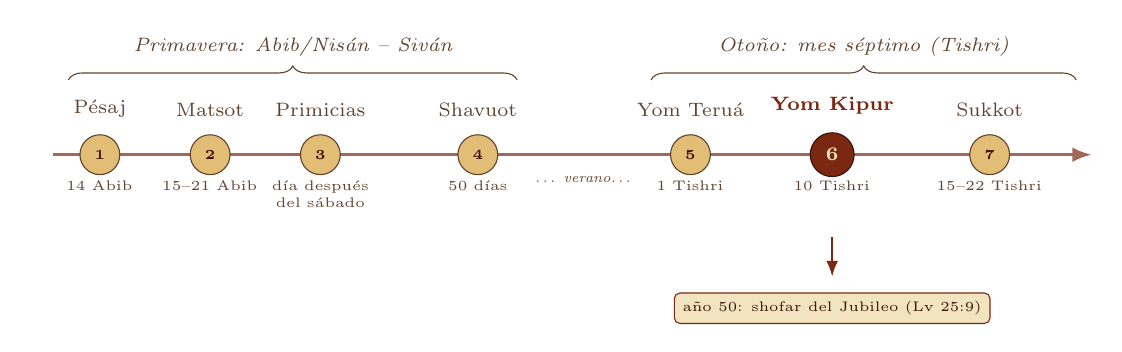
\begin{tikzpicture}[x=1cm,y=1cm,font=\scriptsize]
 \def\fiestaactual{6}
 \draw[line width=1.2pt,tierraroja!70,-{Latex[length=2.5mm]}] (0,0) -- (13.2,0);
 \draw[decorate,decoration={brace,amplitude=5pt},sepia] (0.2,0.95) -- (5.9,0.95) node[midway,above=5pt,font=\scriptsize\itshape]{Primavera: Abib/Nisán -- Siván};
 \draw[decorate,decoration={brace,amplitude=5pt},sepia] (7.6,0.95) -- (13.0,0.95) node[midway,above=5pt,font=\scriptsize\itshape]{Otoño: mes séptimo (Tishri)};
 \foreach \n/\x/\t/\d in {1/0.6/Pésaj/{14 Abib},2/2.0/Matsot/{15--21 Abib},3/3.4/Primicias/{día después del sábado},4/5.4/Shavuot/{50 días},5/8.1/Yom Teruá/{1 Tishri},6/9.9/Yom Kipur/{10 Tishri},7/11.9/Sukkot/{15--22 Tishri}}{
   \ifnum\n=\fiestaactual
     \node[circle,fill=tierraroja,draw=caferojizo,minimum size=5.5mm,text=papiro,font=\scriptsize\bfseries] at (\x,0) {\n};
     \node[above=3pt,font=\scriptsize\bfseries,text=tierraroja] at (\x,0.28) {\t};
   \else
     \node[circle,fill=mostaza!70,draw=sepia,minimum size=4.5mm,text=caferojizo,font=\tiny\bfseries] at (\x,0) {\n};
     \node[above=3pt,text=sepia] at (\x,0.25) {\t};
   \fi
   \node[below=6pt,text width=1.6cm,align=center,font=\tiny,text=sepia] at (\x,0) {\d};}
 \node[font=\tiny\itshape,text=sepia] at (6.75,-0.32) {\ldots\ verano\ldots};
 % agregado de este estudio: el Jubileo se anuncia en Yom Kipur del año 50
 \draw[-{Latex[length=2mm]},tierraroja,line width=0.8pt] (9.9,-1.05) -- (9.9,-1.55);
 \node[draw=tierraroja,fill=papiro,rounded corners=2pt,font=\tiny,text=caferojizo,align=center,inner sep=3pt] at (9.9,-1.95) {año 50: shofar del Jubileo (Lv 25:9)};
\end{tikzpicture}\par
\pie{\textit{Figura 1.} El ciclo de Levítico 23 y el anuncio del Jubileo. \textit{Nota.} Elaboración propia: esquema estándar de la serie; el Jubileo se proclama el 10 de Tishri del año cincuenta.}
\end{minipage}\end{center}

%===================================================================
\section{El texto: Levítico 25 y sus ecos}

\subsection{La cuenta y la proclamación (Lv 25:8--12)}
Levítico 25 empieza en el monte Sinaí (v.~1) y legisla primero el año sabático de la tierra, la \emph{shemitá}: seis años de siembra y un séptimo de ``descanso'' para la tierra (vv.~2--7). Sobre ese ciclo construye el Jubileo, y la cuenta, la fecha y el anuncio caben en tres versículos:

\hebverso{וְסָפַרְתָּ לְךָ שֶׁבַע שַׁבְּתֹת שָׁנִים שֶׁבַע שָׁנִים שֶׁבַע פְּעָמִים \\ וְהַעֲבַרְתָּ שׁוֹפַר תְּרוּעָה בַּחֹדֶשׁ הַשְּׁבִעִי בֶּעָשׂוֹר לַחֹדֶשׁ בְּיוֹם הַכִּפֻּרִים \\ וּקְרָאתֶם דְּרוֹר בָּאָרֶץ לְכָל־יֹשְׁבֶיהָ יוֹבֵל הִוא תִּהְיֶה לָכֶם}
\begin{cita}Y contarás siete semanas de años, siete veces siete años, de modo que los días de las siete semanas de años vendrán a serte cuarenta y nueve años. Entonces harás tocar fuertemente la trompeta en el mes séptimo a los diez días del mes; el día de la expiación haréis tocar la trompeta por toda vuestra tierra. Y santificaréis el año cincuenta, y pregonaréis libertad en la tierra a todos sus moradores; ese año os será de jubileo, y volveréis cada uno a vuestra posesión, y cada cual volverá a su familia.\fuente{(Lv 25:8--10)}\end{cita}

Cuatro verbos ordenan el texto: \emph{contar} (\heb{וְסָפַרְתָּ}), \emph{hacer pasar} el shofar (\heb{וְהַעֲבַרְתָּ}), \emph{santificar} el año (\heb{וְקִדַּשְׁתֶּם}) y \emph{proclamar} la libertad (\heb{וּקְרָאתֶם}). El último es el mismo verbo de las convocaciones santas de Levítico 23, \emph{qará}, de donde viene \emph{mikrá kódesh}. Lo que en Lv 23 se ``proclama'' es un tiempo santo; lo que en Lv 25:10 se proclama es \emph{derór}, la liberación. (En mi presentación sobre el Jubileo anoté que \emph{mikrá} se ha entendido como repaso o ensayo; el sentido léxico es convocación, reunión y también lectura en Neh 8:8, de modo que lo de ensayo vale solo como analogía.) Siguen dos consecuencias en paralelo, ``volveréis cada uno a vuestra posesión, y cada cual volverá a su familia'': el retorno tiene una cara territorial (\emph{ajuzá}, la posesión) y otra social (\emph{mishpajá}, el clan).

Los versículos 11--12 extienden al año cincuenta las reglas agrícolas del sabático (no sembrar, no segar lo que nazca solo, no vendimiar la viña no podada), ``porque es jubileo; santo será a vosotros''. El versículo 13 repite como estribillo: ``En este año de jubileo volveréis cada uno a vuestra posesión''.

\subsection{``La tierra mía es'' (Lv 25:23)}
La regla que sostiene el capítulo es teológica antes que económica. Después de regular las ventas (vv.~14--17) y de prometer que la tierra dará fruto para tres años si Israel obedece (vv.~18--22), Dios da la razón de todo el sistema:

\hebverso{וְהָאָרֶץ לֹא תִמָּכֵר לִצְמִתֻת כִּי־לִי הָאָרֶץ כִּי־גֵרִים וְתוֹשָׁבִים אַתֶּם עִמָּדִי}
\begin{cita}La tierra no se venderá a perpetuidad, porque la tierra mía es; pues vosotros forasteros y extranjeros sois para conmigo. Por tanto, en toda la tierra de vuestra posesión otorgaréis rescate a la tierra.\fuente{(Lv 25:23--24)}\end{cita}

El israelita no es dueño absoluto de su campo. Es un \emph{guer} y un \emph{toshav}, un residente a quien el Dueño ha cedido el uso, y por eso lo que se ``vende'' son las cosechas hasta el Jubileo, no la tierra: ``conforme al número de los años de los frutos te venderá él a ti'' (v.~15). Por la misma razón cada venta queda sujeta a \emph{ge'ulá}, rescate (v.~24). El salmista dirá lo mismo en primera persona, ``forastero soy para ti, y advenedizo, como todos mis padres'' (Sal 39:12 [39:13]), y David en la oración de las ofrendas para el templo: ``extranjeros y advenedizos somos delante de ti'' (1~Cr 29:15).

\subsection{Las reglas: tierra, casas y personas (Lv 25:14--55)}
El resto del capítulo despliega el principio en una serie de casos.

\paragraph{Ventas sin engaño (vv.~14--17).} ``Y cuando vendiereis algo a vuestro prójimo, o comprareis de mano de vuestro prójimo, no engañe ninguno a su hermano'' (v.~14). El precio se calcula por los años que faltan hasta el Jubileo: ``cuanto mayor fuere el número de los años, aumentarás el precio, y cuanto menor fuere el número, disminuirás el precio; porque según el número de las cosechas te venderá él'' (v.~16). El verbo \heb{תּוֹנוּ} (\emph{tonú}, de \emph{yaná}, ``oprimir, defraudar'') vuelve en el v.~17 con su contrapeso, ``sino temed a vuestro Dios''. La Figura~2 muestra el efecto económico de la regla.

\begin{center}\begin{minipage}{\linewidth}\centering
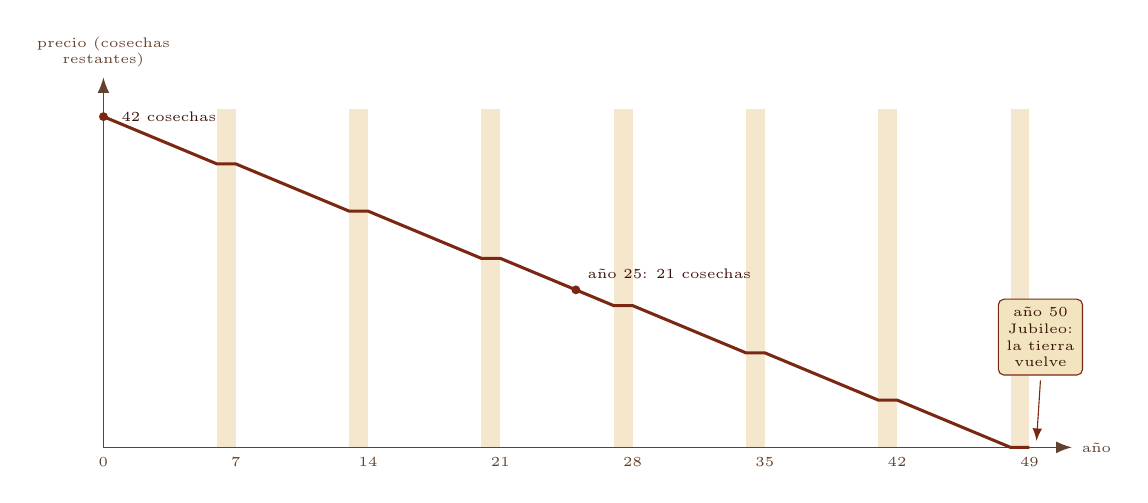
\begin{tikzpicture}[x=1cm,y=1cm,font=\scriptsize]
 \draw[sepia,line width=0.5pt,-{Latex[length=2mm]}] (0,0) -- (12.3,0) node[right,font=\tiny,text=sepia] {año};
 \draw[sepia,line width=0.5pt,-{Latex[length=2mm]}] (0,0) -- (0,4.7) node[above,font=\tiny,text=sepia,align=center] {precio (cosechas\\ restantes)};
 \foreach \k in {7,14,21,28,35,42,49}{
   \fill[mostaza!25] ({(\k-1)*0.24},0) rectangle ({\k*0.24},4.3);
   \node[below,font=\tiny,text=sepia] at ({\k*0.24},0) {\k};}
 \node[below,font=\tiny,text=sepia] at (0,0) {0};
 \draw[tierraroja,line width=1.1pt] plot coordinates {(0.00,4.20) (0.24,4.10) (0.48,4.00) (0.72,3.90) (0.96,3.80) (1.20,3.70) (1.44,3.60) (1.68,3.60) (1.92,3.50) (2.16,3.40) (2.40,3.30) (2.64,3.20) (2.88,3.10) (3.12,3.00) (3.36,3.00) (3.60,2.90) (3.84,2.80) (4.08,2.70) (4.32,2.60) (4.56,2.50) (4.80,2.40) (5.04,2.40) (5.28,2.30) (5.52,2.20) (5.76,2.10) (6.00,2.00) (6.24,1.90) (6.48,1.80) (6.72,1.80) (6.96,1.70) (7.20,1.60) (7.44,1.50) (7.68,1.40) (7.92,1.30) (8.16,1.20) (8.40,1.20) (8.64,1.10) (8.88,1.00) (9.12,0.90) (9.36,0.80) (9.60,0.70) (9.84,0.60) (10.08,0.60) (10.32,0.50) (10.56,0.40) (10.80,0.30) (11.04,0.20) (11.28,0.10) (11.52,0.00) (11.76,0.00)};
 \fill[tierraroja] (0,4.2) circle (1.6pt) node[right=3pt,font=\tiny,text=caferojizo] {42 cosechas};
 \fill[tierraroja] (6.0,2.0) circle (1.6pt) node[above right=1pt,font=\tiny,text=caferojizo] {año 25: 21 cosechas};
 \node[draw=tierraroja,fill=papiro,rounded corners=2pt,font=\tiny,text=caferojizo,align=center,inner sep=3pt] at (11.9,1.4) {año 50\\ Jubileo:\\ la tierra\\ vuelve};
 \draw[-{Latex[length=1.6mm]},tierraroja] (11.9,0.85) -- (11.85,0.08);
\end{tikzpicture}\par
\pie{\textit{Figura 2.} El precio de un campo según los años hasta el Jubileo (Lv 25:14--17). \textit{Nota.} Elaboración propia. Se compra el número de cosechas restantes, no la tierra; las bandas marcan los años sabáticos, en los que no hay cosecha. Excluir esos años es la lectura de varios comentaristas (cf. Milgrom, 2001); el texto solo dice ``según el número de las cosechas'' (v.~16).}
\end{minipage}\end{center}

\paragraph{El rescate de la tierra (vv.~25--28).} ``Cuando tu hermano empobreciere, y vendiere algo de su posesión, entonces su pariente más próximo vendrá y rescatará lo que su hermano hubiere vendido'' (v.~25). Aparece aquí el \emph{goel} (\heb{גֹּאֲלוֹ הַקָּרֹב אֵלָיו}, ``su redentor, el cercano a él''). El texto prevé tres salidas, en orden: el rescate por el pariente; el rescate por el propio vendedor si llega a reunir lo necesario, descontando los años ya usados (vv.~26--27); y, si nada de eso ocurre, la devolución gratuita en el Jubileo: ``al jubileo saldrá, y él volverá a su posesión'' (v.~28).

\paragraph{Casas en ciudades amuralladas y en aldeas (vv.~29--31).} La casa en ciudad con muro puede rescatarse durante un año; pasado ese plazo queda ``para siempre'' (\emph{latsmitut}) para el comprador y no sale en el Jubileo. Las casas de aldeas sin muro, en cambio, ``serán estimadas como los terrenos del campo'' y salen en el Jubileo. La distinción deja ver qué protege la ley: no cualquier propiedad, sino el patrimonio agrícola del clan, del que depende la vida de la familia.

\paragraph{Las ciudades levíticas (vv.~32--34).} Los levitas, que no recibieron territorio tribal (Nm 18:20--24), pueden rescatar ``en cualquier tiempo'' sus casas en las ciudades asignadas (Nm 35:1--8; Jos 21), y el ejido de esas ciudades no se vende, ``porque es perpetua posesión de ellos''.

\paragraph{El préstamo sin interés (vv.~35--38).} Cuando el hermano empobrecido ya no tiene qué vender, se le sostiene ``como forastero y extranjero'': ``No tomarás de él usura ni ganancia, sino tendrás temor de tu Dios, y tu hermano vivirá contigo'' (v.~36). La razón es otra vez el éxodo: ``Yo \SENOR{} vuestro Dios, que os saqué de la tierra de Egipto, para daros la tierra de Canaán, para ser vuestro Dios'' (v.~38).

\paragraph{El hermano que se vende (vv.~39--55).} El último grado de la pobreza es venderse a sí mismo. Si el comprador es israelita, ``no le harás servir como esclavo. Como criado, como extranjero estará contigo; hasta el año del jubileo te servirá. Entonces saldrá libre de tu casa; él y sus hijos consigo, y volverá a su familia, y a la posesión de sus padres se restituirá'' (vv.~39--41). Si el comprador es un extranjero residente, la familia tiene derecho de rescate (un hermano, un tío, el hijo del tío o cualquier pariente cercano), o él mismo, si prospera (vv.~47--49). En ambos casos el fundamento es el mismo:

\hebverso{כִּי־עֲבָדַי הֵם אֲשֶׁר־הוֹצֵאתִי אֹתָם מֵאֶרֶץ מִצְרָיִם לֹא יִמָּכְרוּ מִמְכֶּרֶת עָבֶד}
\begin{cita}Porque son mis siervos, los cuales saqué yo de la tierra de Egipto; no serán vendidos a manera de esclavos.\fuente{(Lv 25:42)}\end{cita}

El capítulo termina con la misma frase, ampliada como sello: ``Porque mis siervos son los hijos de Israel; son siervos míos, a los cuales saqué de la tierra de Egipto. Yo \SENOR{} vuestro Dios'' (v.~55). Un israelita no puede ser posesión definitiva de otro, porque ya tiene dueño.

\begin{nota}[Precisión]
Los vv.~44--46 permiten comprar siervos de las naciones vecinas y de los extranjeros residentes, y tenerlos ``por posesión'' (\emph{ajuzá}) sin salida en el Jubileo. La ley del Jubileo protege, en su letra, al israelita. Los comentarios lo señalan como un límite real del texto (Milgrom, 2001; Hartley, 1992); los profetas ampliarán el horizonte: el siervo del \SENOR{} es ``luz de las naciones'' para ``que saques de la cárcel a los presos'' (Is 42:6--7), y el extranjero y el eunuco que se allegan al \SENOR{} reciben lugar en su casa, ``casa de oración para todos los pueblos'' (Is 56:3--7).
\end{nota}

\begin{center}\begin{minipage}{\linewidth}\centering
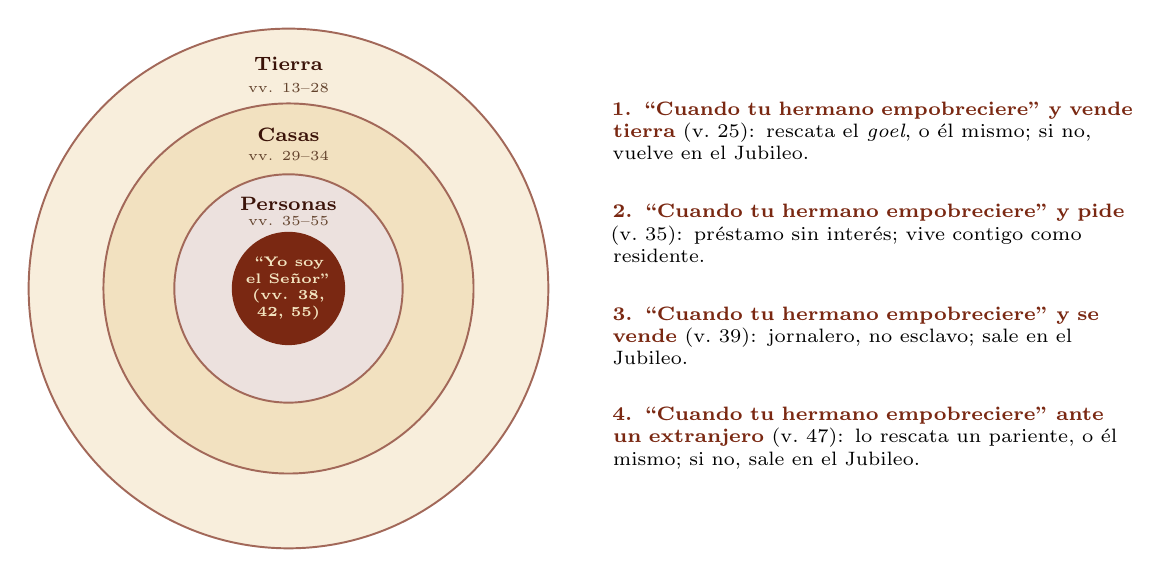
\begin{tikzpicture}[x=1cm,y=1cm,font=\scriptsize]
 \foreach \r/\c in {3.3/mostaza!18, 2.35/mostaza!32, 1.45/tierraroja!14}{\fill[\c] (0,0) circle (\r);}
 \foreach \r in {3.3,2.35,1.45}{\draw[tierraroja!70,line width=0.7pt] (0,0) circle (\r);}
 \fill[tierraroja] (0,0) circle (0.72);
 \node[text=papiro,font=\tiny\bfseries,align=center] at (0,0) {``Yo soy\\ el \SENOR''\\ (vv. 38,\\ 42, 55)};
 \node[font=\scriptsize\bfseries,text=caferojizo] at (0,2.85) {Tierra};
 \node[font=\tiny,text=sepia] at (0,2.55) {vv. 13--28};
 \node[font=\scriptsize\bfseries,text=caferojizo] at (0,1.95) {Casas};
 \node[font=\tiny,text=sepia] at (0,1.68) {vv. 29--34};
 \node[font=\scriptsize\bfseries,text=caferojizo] at (0,1.07) {Personas};
 \node[font=\tiny,text=sepia] at (0,0.86) {vv. 35--55};
 % leyendas a la derecha
 \node[anchor=west,text width=6.6cm,align=left,font=\scriptsize] at (4.0,2.0) {\textbf{\textcolor{tierraroja}{1. ``Cuando tu hermano empobreciere'' y vende tierra}} (v.~25): rescata el \emph{goel}, o él mismo; si no, vuelve en el Jubileo.};
 \node[anchor=west,text width=6.6cm,align=left,font=\scriptsize] at (4.0,0.7) {\textbf{\textcolor{tierraroja}{2. ``Cuando tu hermano empobreciere'' y pide}} (v.~35): préstamo sin interés; vive contigo como residente.};
 \node[anchor=west,text width=6.6cm,align=left,font=\scriptsize] at (4.0,-0.6) {\textbf{\textcolor{tierraroja}{3. ``Cuando tu hermano empobreciere'' y se vende}} (v.~39): jornalero, no esclavo; sale en el Jubileo.};
 \node[anchor=west,text width=6.6cm,align=left,font=\scriptsize] at (4.0,-1.9) {\textbf{\textcolor{tierraroja}{4. ``Cuando tu hermano empobreciere'' ante un extranjero}} (v.~47): lo rescata un pariente, o él mismo; si no, sale en el Jubileo.};
\end{tikzpicture}\par
\pie{\textit{Figura 3.} Levítico 25 en círculos de redención: tierra, casas y personas. \textit{Nota.} Elaboración propia. Los cuatro casos se abren con la misma fórmula, \heb{כִּי־יָמוּךְ אָחִיךָ} (vv.~25, 35, 39; en v.~47 \heb{וּמָךְ אָחִיךָ}); la división en tres grados de pobreza sigue a Milgrom (2001). La disposición en círculos es una propuesta de lectura.}
\end{minipage}\end{center}

\subsection{Los textos del Jubileo: tabla sinóptica}
El Jubileo no está aislado: se apoya en las leyes de la liberación del siervo hebreo y del año sabático, reaparece en otras leyes del Pentateuco y deja huellas en la narración y en los profetas. Las Tablas 1 y 2 recogen qué añade cada texto.

\begin{center}\begin{minipage}{\linewidth}\centering\small\renewcommand{\arraystretch}{1.18}
\begin{tabular}{@{}L{2.4cm}L{4.6cm}L{7.6cm}@{}}
\toprule
\textbf{Texto} & \textbf{Tema} & \textbf{Qué añade} \\ \midrule
Éx 21:2--6 & Siervo hebreo & Sirve seis años y sale libre el séptimo; si decide quedarse, sirve ``para siempre'' (\heb{לְעֹלָם}). \\
Éx 23:10--11 & Año séptimo de la tierra & La tierra descansa ``para que coman los pobres de tu pueblo''. \\
Lv 25:1--7 & \emph{Shemitá} & ``la tierra tendrá descanso, reposo para \SENOR'' (\emph{shabat shabatón}); lo que nace solo es para todos. \\
Lv 25:8--12 & Cuenta y anuncio & 7\,×\,7 años; shofar el 10 del mes séptimo, Día de la Expiación; \emph{derór}; retorno a posesión y familia. \\
Lv 25:13--28 & Tierra & Precio según los años; ``la tierra mía es''; \emph{ge'ulá}; el \emph{goel}; devolución en el Jubileo. \\
Lv 25:29--34 & Casas y levitas & Casa amurallada: rescate de un año; aldeas como el campo; derechos levíticos perpetuos. \\
Lv 25:35--55 & Personas & Préstamo sin interés; el hermano vendido sirve como jornalero hasta el Jubileo; rescate por la familia. \\
Lv 26:34--35, 43 & Sábados de la tierra & Si Israel no guarda los reposos, la tierra los ``gozará'' durante el exilio. \\
Lv 27:16--25 & Campos consagrados & Valor según los años hasta el Jubileo; en el Jubileo el campo vuelve ``a aquel de quien él la compró'' (v.~24). \\
Nm 36:1--12 & Hijas de Zelofehad & El Jubileo no corrige una herencia pasada por matrimonio a otra tribu (v.~4): deben casarse dentro de su tribu. \\
Dt 15:1--18 & \emph{Shemitá} de deudas & ``Remisión'' (\heb{שְׁמִטָּה}) de préstamos el año séptimo; liberación del siervo con provisiones. \\
\bottomrule
\end{tabular}\par
\pie{\textit{Tabla 1.} Textos legislativos del Jubileo y del año sabático. \textit{Nota.} Elaboración propia con la BHS y la RVR1960.}
\end{minipage}\end{center}

\begin{center}\begin{minipage}{\linewidth}\centering\small\renewcommand{\arraystretch}{1.18}
\begin{tabular}{@{}L{2.4cm}L{4.6cm}L{7.6cm}@{}}
\toprule
\textbf{Texto} & \textbf{Tema} & \textbf{Qué añade} \\ \midrule
Rut 2--4 & Booz, el \emph{goel} & Rescate del campo de Elimelec y matrimonio con Rut ante los ancianos, en la puerta; nace Obed, abuelo de David. \\
1~R 21:1--16 & La viña de Nabot & ``Guárdeme \SENOR{} de que yo te dé a ti la heredad de mis padres'' (v.~3): la \emph{najalá} no se vende. \\
Jer 32:6--15 & Jeremías redime Anatot & Durante el asedio compra, como pariente con derecho de rescate, el campo de su primo: ``Aún se comprarán casas, heredades y viñas'' (v.~15). \\
Jer 34:8--22 & El \emph{derór} de Sedequías & Pacto de liberar a los siervos hebreos, luego revocado; Dios ``promulga libertad'' a la espada (v.~17). \\
Ez 46:16--18 & El príncipe & Lo que el príncipe da a un siervo es suyo ``hasta el año del jubileo'' (RVR1960; lit. ``el año de la libertad'', \heb{שְׁנַת הַדְּרוֹר}); no puede despojar al pueblo de su heredad. \\
Neh 5:1--13; 10:31 & Crisis de deudas & Nehemías obliga a devolver campos, viñas y casas; el pueblo jura guardar el año séptimo y la remisión de deudas. \\
Is 49:8--9 & El siervo y la tierra & ``En tiempo aceptable te oí''; restaurar la tierra, heredar heredades asoladas, decir a los presos: ``Salid''. \\
Is 58:6 & El ayuno verdadero & ``Dejar ir libres a los quebrantados'': lenguaje de liberación en un texto sobre el ayuno. \\
Is 61:1--3 & El ungido & Proclamar \emph{derór} a los cautivos, ``el año de la buena voluntad'' (\emph{shenat ratsón}) y ``el día de venganza''. \\
Dn 9:24--27 & Setenta semanas & 70\,×\,7 = 490 años, diez veces cuarenta y nueve: una cronología en clave de semanas de años. \\
Lc 4:16--21 & Nazaret & Jesús lee Is 61:1--2 con Is 58:6 y declara: ``Hoy se ha cumplido esta Escritura''. \\
\bottomrule
\end{tabular}\par
\pie{\textit{Tabla 2.} Ecos narrativos y proféticos del Jubileo. \textit{Nota.} Elaboración propia. La relación de Dn 9 con el Jubileo es una lectura (véase §5.5).}
\end{minipage}\end{center}

\begin{nota}[Precisión: el siervo hebreo, ¿seis años o hasta el Jubileo?]
Éxodo 21:2 y Deuteronomio 15:12 liberan al siervo hebreo al séptimo año de servicio; Levítico 25:40 lo hace servir ``hasta el año del jubileo''. La crítica histórica suele ver aquí leyes de épocas distintas (Fager, 1993). La tradición judía las armoniza: Lv 25 trataría del israelita que se vende por pobreza extrema, y el ``para siempre'' del siervo que se perfora la oreja (Éx 21:6) significaría ``hasta el Jubileo'' (Rashi a Éx 21:6, siguiendo a la \emph{Mejiltá}). Otros intérpretes sostienen que Lv 25 no anula la liberación del séptimo año, sino que pone un tope absoluto: nadie queda sujeto más allá del Jubileo (Wright, 2004).
\end{nota}

%===================================================================
\section{Lectura histórica}

\subsection{Tierra, clan y herencia en Israel}
La ley del Jubileo supone una sociedad agraria organizada en tres niveles: la tribu (\emph{shévet} o \emph{maté}), el clan (\emph{mishpajá}) y la casa paterna (\emph{bet av}). La tierra se repartió ``por suerte'' a cada tribu y, dentro de ella, a cada clan (Nm 26:52--56; 33:54; Jos 13--19). Ese reparto era una herencia, no un mercado; la palabra es \emph{najalá} (\heb{נַחֲלָה}), la porción recibida que pasa de padres a hijos. Por eso el hito narrado detrás del Jubileo es la entrada en Canaán y el reparto de la tierra, que Levítico 25:2 pone como condición: ``Cuando hayáis entrado en la tierra que yo os doy''.

La historia de Nabot muestra la fuerza de esa idea. Cuando Acab le ofrece comprar su viña o cambiarla por otra mejor, Nabot responde: ``Guárdeme \SENOR{} de que yo te dé a ti la heredad de mis padres'' (1~R 21:3). Acab y Jezabel no pueden comprarla y la obtienen con un juicio falso. Los profetas del siglo VIII denuncian el mismo fenómeno a escala social: ``¡Ay de los que juntan casa a casa, y añaden heredad a heredad hasta ocuparlo todo!'' (Is 5:8); ``codician las heredades, y las roban; y casas, y las toman; oprimen al hombre y a su casa, al hombre y a su heredad'' (Mi 2:2). La ley de los linderos protege lo mismo: ``No reducirás los límites de la propiedad de tu prójimo'' (Dt 19:14; cf. Pr 23:10--11, donde el defensor del huérfano es su \emph{goel}).

El folleto de Wight sobre usos y costumbres, que he consultado a lo largo de la serie, describe la vida de aldea en que se inscribe esta ley: el campo familiar, las piedras de lindero, la puerta de la ciudad como lugar de los contratos y de los ancianos (Wight, 1953). El libro de Rut lo muestra en acción cuando Booz se sienta ``a la puerta'' con diez ancianos para resolver el rescate del campo de Elimelec (Rut 4:1--2).

\subsection{Los edictos de remisión del antiguo Cercano Oriente}
Israel no inventó la idea de una liberación periódica de deudas. En Mesopotamia, desde el tercer milenio, los reyes proclamaban ocasionalmente un \emph{mīšarum} (``rectitud, justicia'') o un \emph{andurārum} (``liberación''): cancelaban deudas de consumo, liberaban a los esclavos por deudas y devolvían tierras empeñadas. El caso mejor conservado es el edicto de Ammi-ṣaduqa de Babilonia (siglo XVII a.\,e.\,c.), que anula deudas atrasadas y libera a quienes habían sido vendidos por deudas, con excepciones para los préstamos comerciales. La expresión babilónica para establecer tal edicto, \emph{mīšaram šakānum}, ``establecer la justicia'', tiene un eco cercano en el par hebreo \emph{mishpat utsedaká}, ``juicio y justicia'' (Weinfeld, 1995).

El parentesco léxico es directo, pues el acadio \emph{andurārum} y el hebreo \emph{derór} son cognados. Weinfeld (1995) mostró que la expresión ``proclamar \emph{derór}'' corresponde a la fórmula real mesopotámica y que la pareja ``justicia y rectitud'' de los profetas tiene ese trasfondo social; Lemche (1979) estudió la aplicación real de esos edictos y su carácter irregular.

\begin{nota}[Precisión: semejanzas y diferencias]
El paralelo ilumina, pero no explica todo. Los edictos mesopotámicos eran decisiones del rey, a menudo al subir al trono, sin periodicidad fija y con fines también políticos. El Jubileo de Levítico es periódico (cada cincuenta años), no depende del rey sino de Dios, se proclama en un día cultual (el Día de la Expiación) y se funda en dos afirmaciones teológicas: la tierra es de Dios y el pueblo es su siervo rescatado de Egipto (Lv 25:23, 42). La tierra no vuelve al estado ni al templo, sino a la familia. Weinfeld (1995) y Bergsma (2007) insisten en las dos caras: el trasfondo común y la transformación israelita.
\end{nota}

\subsection{¿Se practicó el Jubileo?}
Ningún relato bíblico narra la celebración de un año de Jubileo. Los textos que más se acercan muestran otras instituciones, o bien la ruptura de la ley:
\begin{itemize}\setlength{\itemsep}{1pt}
\item \textbf{Jeremías 34:8--22.} Durante el asedio babilónico (ca. 588 a.\,e.\,c.), Sedequías hace un pacto ``para promulgarles libertad'' (\heb{לִקְרֹא לָהֶם דְּרוֹר}): cada uno debía dejar ir libre a su siervo hebreo. Cuando el asedio se levanta por un tiempo, los amos vuelven a tomar a los liberados. El profeta cita la ley del séptimo año (Jer 34:14; cf. Dt 15:12), pero usa el vocabulario de Lv 25:10. Se trata de un \emph{derór} proclamado al modo de un edicto real, más que de un Jubileo calendárico (Lundbom, 2004).
\item \textbf{Nehemías 5:1--13.} Ante una crisis de deudas que obligaba a vender hijos e hijas y a empeñar campos, Nehemías exige devolver ``sus tierras, sus viñas, sus olivares y sus casas''; de nuevo una remisión extraordinaria. En Neh 10:31 [10:32] el pueblo se compromete a guardar el año séptimo y a remitir ``toda deuda''.
\item \textbf{2~Crónicas 36:21.} El exilio duró ``hasta que la tierra hubo gozado de reposo'', citando Lv 26:34--35 y Jer 25:11: el cronista interpreta los setenta años como sábados no guardados.
\item \textbf{El año sabático, en cambio, sí está atestiguado} en el Segundo Templo (1~Mac 6:49, 53; Josefo, \emph{Antigüedades} 14.475; 15.7).
\end{itemize}

El Talmud conserva una tradición según la cual el Jubileo dejó de regir cuando las tribus de Rubén, Gad y la media tribu de Manasés fueron desterradas, porque la ley exige ``a todos sus moradores'' (Lv 25:10), es decir, todo Israel en su tierra (b.~\emph{Arajin} 32b; cf. \emph{Sifra}, \emph{Behar}). Se trata de una explicación posterior del silencio, y no de un dato de archivo.

Los especialistas se dividen.
\begin{itemize}\setlength{\itemsep}{1pt}
\item \textbf{Una ley ideal o tardía.} De Vaux (1985) consideró el Jubileo una ley de carácter utópico, nunca aplicada de manera regular, que sistematiza el año sabático. Fager (1993) lo lee como una propuesta sacerdotal posterior al exilio para reorganizar la tenencia de la tierra en la comunidad que volvía.
\item \textbf{Raíces antiguas.} Milgrom (2001) sostiene que la ley tiene raíces preexílicas y la relaciona con la crisis agraria del siglo VIII, la misma que denuncian Isaías y Miqueas. Bergsma (2007) concluye que la legislación refleja una sociedad tribal y agraria anterior al exilio, y sigue su relectura hasta Qumrán. Wright (2004) subraya que la ley presupone la organización por clanes de Josué 13--19, que no corresponde al Israel del exilio.
\end{itemize}
El silencio de las fuentes no prueba que la ley no existiera. Muestra, al menos, que su cumplimiento fue difícil y que los profetas la recordaron como deuda pendiente.

\subsection{El Jubileo en el Segundo Templo}
Después del exilio, el Jubileo pasó a ser una manera de medir la historia.

\paragraph{El Libro de los Jubileos} (siglo II a.\,e.\,c.) reescribe Génesis y el comienzo de Éxodo y divide toda la historia en jubileos de cuarenta y nueve años, subdivididos en ``semanas de años''. Su cronología culmina en la entrada en Canaán al cumplirse cincuenta jubileos desde la creación (Jub 50:4): la tierra prometida llega en un ``Jubileo de jubileos'' (VanderKam, 2001). El libro defiende además un calendario solar de 364 días, que comparte con algunos textos de Qumrán (VanderKam, 1998).

\paragraph{11QMelquisedec (11Q13).} Este texto de la cueva 11 de Qumrán (siglo I a.\,e.\,c.) combina Levítico 25:13, Deuteronomio 15:2 e Isaías 61:1 y anuncia que en los últimos días Melquisedec, figura celestial, proclamará la liberación (\emph{derór}) a los cautivos, para ``liberarlos de la deuda de todas sus iniquidades''. El acontecimiento sucede ``en la primera semana del jubileo que sigue a los nueve jubileos'', y el texto dice que ``el día de la expiación'' es el final del décimo jubileo, cuando se hará expiación por todos los hijos de la luz (García Martínez, 1992; Vermes, 2004; Kobelski, 1981). El testimonio pesa mucho para este estudio, porque muestra que un siglo antes de Jesús un grupo judío ya leía juntos Levítico 25 e Isaías 61 y vinculaba la liberación final con el Día de la Expiación, el mismo puente que une este capítulo con el de Yom Kipur.

\paragraph{Josefo y Filón.} Josefo describe el Jubileo como el año en que los deudores quedan libres y las tierras vuelven a sus dueños, y explica que el nombre significa ``libertad'' (\emph{Antigüedades} 3.280--286). Filón lo interpreta como una ley de humanidad que enseña que la tierra pertenece a Dios (\emph{De specialibus legibus} 2.110--123).

\subsection{Usos posteriores del término}
El nombre siguió vivo fuera de su marco original. En el año 1300, el papa Bonifacio VIII proclamó el primer ``año santo'' o ``jubileo'' de la Iglesia romana, con indulgencias para los peregrinos a Roma; la costumbre se mantiene con intervalos de veinticinco años. En 1751 la asamblea de Pensilvania encargó una campana para el quincuagésimo aniversario de la Carta de Privilegios de 1701, y le hizo grabar Levítico 25:10: \emph{Proclaim liberty throughout all the land unto all the inhabitants thereof} (``Pregonad libertad por toda la tierra a todos sus habitantes''). Se trata de la Campana de la Libertad de Filadelfia, que más tarde se convirtió en símbolo de los abolicionistas (Nash, 2010).

\begin{nota}[Precisión]
El ``jubileo'' católico de 1300 y la campana de 1751 son usos posteriores del término, no interpretaciones del texto: el primero aplica la palabra a un perdón eclesiástico de penas; la segunda, a un aniversario civil de cincuenta años y luego a la causa de la abolición. Se mencionan como historia de la recepción.
\end{nota}

\begin{center}\begin{minipage}{\linewidth}\centering
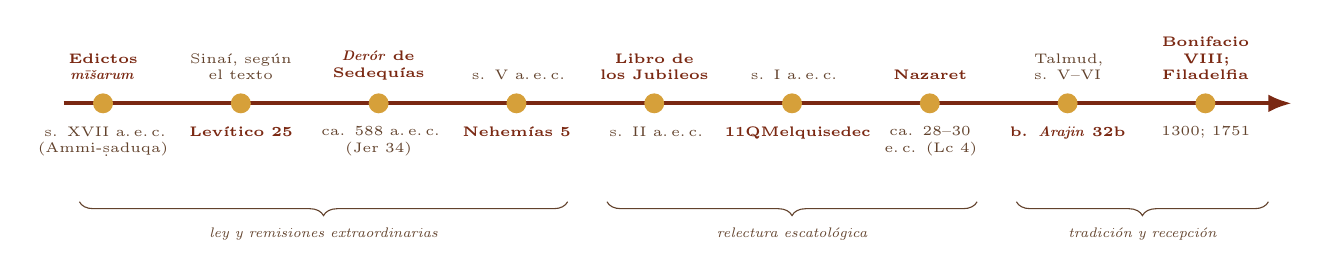
\begin{tikzpicture}[x=1cm,y=1cm,font=\scriptsize]
 \draw[line width=1.5pt,tierraroja,-{Latex[length=3mm]}] (0,0) -- (15.6,0);
 \foreach \x/\a/\b/\p in {0.5/{Edictos \emph{mīšarum}}/{s. XVII a.\,e.\,c. (Ammi-ṣaduqa)}/1,
                         2.25/{Levítico 25}/{Sinaí, según el texto}/0,
                         4.0/{\emph{Derór} de Sedequías}/{ca. 588 a.\,e.\,c. (Jer 34)}/1,
                         5.75/{Nehemías 5}/{s. V a.\,e.\,c.}/0,
                         7.5/{Libro de los Jubileos}/{s. II a.\,e.\,c.}/1,
                         9.25/{11QMelquisedec}/{s. I a.\,e.\,c.}/0,
                         11.0/{Nazaret}/{ca. 28--30 e.\,c. (Lc 4)}/1,
                         12.75/{b. \emph{Arajin} 32b}/{Talmud, s. V--VI}/0,
                         14.5/{Bonifacio VIII; Filadelfia}/{1300; 1751}/1}{
   \fill[mostaza] (\x,0) circle (3.6pt);
   \ifnum\p=1
     \node[above=5pt,text width=1.68cm,align=center,font=\tiny\bfseries,text=tierraroja] at (\x,0) {\a};
     \node[below=5pt,text width=1.68cm,align=center,font=\tiny,text=sepia] at (\x,0) {\b};
   \else
     \node[above=5pt,text width=1.68cm,align=center,font=\tiny,text=sepia] at (\x,0) {\b};
     \node[below=5pt,text width=1.68cm,align=center,font=\tiny\bfseries,text=tierraroja] at (\x,0) {\a};
   \fi}
 \draw[decorate,decoration={brace,amplitude=5pt,mirror},sepia] (0.2,-1.25) -- (6.4,-1.25) node[midway,below=6pt,font=\tiny\itshape,text=sepia] {ley y remisiones extraordinarias};
 \draw[decorate,decoration={brace,amplitude=5pt,mirror},sepia] (6.9,-1.25) -- (11.6,-1.25) node[midway,below=6pt,font=\tiny\itshape,text=sepia] {relectura escatológica};
 \draw[decorate,decoration={brace,amplitude=5pt,mirror},sepia] (12.1,-1.25) -- (15.3,-1.25) node[midway,below=6pt,font=\tiny\itshape,text=sepia] {tradición y recepción};
\end{tikzpicture}\par
\pie{\textit{Figura 4.} El Jubileo en la historia. \textit{Nota.} Elaboración propia. Fechas aproximadas; la datación de Levítico 25 es discutida (véase §3.3).}
\end{minipage}\end{center}

%===================================================================
\section{Lectura filológica}

El vocabulario del Jubileo es pequeño y preciso. Unas pocas palabras hebreas sostienen la institución: el nombre del año (\emph{yovel}), su contenido (\emph{derór}), el procedimiento (\emph{ge'ulá}) y su agente (\emph{goel}), el objeto (\emph{ajuzá}, \emph{najalá}) y el fundamento (\emph{tsemitut}, \emph{guer ve-toshav}). La Septuaginta las vertió con palabras que el Nuevo Testamento usará después para hablar del perdón y del rescate.

\begin{filologia}[\emph{yovel}, ``cuerno de carnero'', ``jubileo'']
\begin{tabular}{@{}L{3.3cm}L{1.4cm}L{9.85cm}@{}}
\heb{יוֹבֵל} \emph{yovel} & \heb{יבל} & Sustantivo masculino; 27 veces en el AT (conteo propio): 20 en Lv 25 y 27, 5 en Jos 6 (las bocinas de carnero), más Éx 19:13 y Nm 36:4. Su sentido básico parece ser ``carnero'' y, por extensión, el cuerno del carnero usado como instrumento. \\[2pt]
\heb{שׁוֹפְרוֹת הַיּוֹבְלִים} & & ``Bocinas de cuernos de carnero'' (Jos 6:4): los siete shofares que rodean Jericó. ``Y cuando toquen prolongadamente el cuerno de carnero'' (\heb{בִּמְשֹׁךְ בְּקֶרֶן הַיּוֹבֵל}, Jos 6:5). \\[2pt]
\heb{בִּמְשֹׁךְ הַיֹּבֵל} & & ``Cuando suene largamente la bocina'' (Éx 19:13): la señal para subir al Sinaí. \\[2pt]
\heb{שְׁנַת הַיּוֹבֵל} & & ``El año del jubileo'' (Lv 25:13; 27:17--24): el año recibe el nombre del cuerno que lo anuncia. \\[2pt]
Etimología & & Discutida. La derivación de ``carnero'' (atestiguada en fenicio) es la más común (\emph{HALOT}); otros la relacionan con \emph{yaval}, ``conducir, llevar'' (el año que ``trae de vuelta''). El latín \emph{iubilaeus} de la Vulgata se cruzó con \emph{iubilare}, ``gritar de alegría'': de ahí el sentido castellano de ``júbilo'', que no está en el hebreo. \\
\end{tabular}
\end{filologia}

\begin{filologia}[\emph{derór}, ``liberación'']
\begin{tabular}{@{}L{3.3cm}L{1.4cm}L{9.85cm}@{}}
\heb{דְּרוֹר} \emph{derór} & \heb{דרר} & Siete veces en el sentido de ``liberación'' (conteo propio; el lema aparece ocho veces, pero en Éx 30:23 califica a la mirra, \emph{mor derór}): Lv 25:10; Is 61:1; Jer 34:8, 15, 17 (dos veces); Ez 46:17. Siempre con el verbo \emph{qará}, ``proclamar'', salvo en Ezequiel. \\[2pt]
\heb{וּקְרָאתֶם דְּרוֹר} & & ``Pregonaréis libertad'' (Lv 25:10): no se describe un sentimiento sino un acto jurídico público. \\[2pt]
\heb{לִקְרֹא לִשְׁבוּיִם דְּרוֹר} & & ``A publicar libertad a los cautivos'' (Is 61:1): el ungido asume la función del heraldo del Jubileo. \\[2pt]
\heb{שְׁנַת הַדְּרוֹר} & & ``El año de la libertad'' (Ez 46:17, lit.; la RVR1960 traduce ``el año del jubileo''): otro nombre del Jubileo. \\[2pt]
Cognado acadio & & \emph{andurārum}, ``liberación'' de deudas y esclavos, en los edictos reales (Weinfeld, 1995). \\[2pt]
Homónimos & & \heb{דְּרוֹר} ``golondrina'' (Sal 84:3 [84:4]; Pr 26:2), el pájaro que vuela libre; \heb{מָר־דְּרוֹר} ``mirra que corre'' (Éx 30:23). La relación con ``liberación'' es posible, pero no segura. \\
\end{tabular}
\end{filologia}

\begin{filologia}[\emph{ge'ulá} y \emph{goel}, ``rescate'' y ``redentor'']
\begin{tabular}{@{}L{3.3cm}L{1.4cm}L{9.85cm}@{}}
\heb{גָּאַל} \emph{ga'al} & \heb{גאל} & ``Rescatar, recobrar'' lo que pertenece a la familia: un campo (Lv 25:25), una casa (v.~29), una persona (vv.~48--49), un objeto consagrado (Lv 27:13--31). \\[2pt]
\heb{גְּאֻלָּה} \emph{ge'ulá} & & ``Rescate'', derecho y precio de rescate (Lv 25:24, 26, 29, 31, 32, 48; Rut 4:6--7; Jer 32:7--8). \\[2pt]
\heb{גֹּאֵל} \emph{goel} & & Participio: ``el que rescata'', el pariente cercano con derecho y deber de rescatar (Lv 25:25; Rut 2:20; 3:9, 12; 4:1--14). \\[2pt]
\heb{גֹּאֵל הַדָּם} & & ``El vengador de la sangre'' (Nm 35:12, 19--27; Dt 19:6, 12): el mismo pariente que restituye la vida de la familia persiguiendo al homicida. \\[2pt]
Dios como \emph{goel} & & ``Os redimiré con brazo extendido'' (\heb{וְגָאַלְתִּי}, Éx 6:6); ``tu Redentor, el Santo de Israel'' (Is 41:14; 43:14); ``\SENOR{} Rey de Israel, y su Redentor'' (Is 44:6); ``Yo sé que mi Redentor vive'' (Job 19:25). \\[2pt]
\emph{Padá} frente a \emph{ga'al} & \heb{פדה} & \emph{Padá} es ``rescatar mediante pago'', sin exigir parentesco (los primogénitos, Éx 13:13). \emph{Ga'al} añade el vínculo familiar: rescata quien tiene derecho porque es pariente. \\
\end{tabular}
\end{filologia}

\begin{filologia}[\emph{ajuzá} y \emph{najalá}, ``posesión'' y ``heredad'']
\begin{tabular}{@{}L{3.3cm}L{1.4cm}L{9.85cm}@{}}
\heb{אֲחֻזָּה} \emph{ajuzá} & \heb{אחז} & De \emph{ajaz}, ``asir, agarrar'': lo que uno tiene tomado. Palabra clave de Lv 25 (vv.~10, 13, 24, 25, 27, 28, 32--34, 41, 45--46): ``volveréis cada uno a vuestra posesión''. En Gn 17:8, ``en heredad perpetua'' (\heb{לַאֲחֻזַּת עוֹלָם}), promesa a Abraham. \\[2pt]
\heb{נַחֲלָה} \emph{najalá} & \heb{נחל} & ``Heredad'': la porción asignada por suerte que pasa de generación en generación (Nm 26:52--56; 36:4; 1~R 21:3). Israel mismo es ``la heredad'' de Dios (Dt 32:9). \\[2pt]
\heb{מִשְׁפָּחָה} \emph{mishpajá} & \heb{שׁפח} & ``Familia, clan'': el grupo de parentesco que sostiene el derecho de rescate (Lv 25:10, 41, 49). \\
\end{tabular}
\end{filologia}

\begin{filologia}[\emph{tsemitut}, \emph{guer} y \emph{toshav}]
\begin{tabular}{@{}L{3.3cm}L{1.4cm}L{9.85cm}@{}}
\heb{לִצְמִתֻת} \emph{litsmitut} & \heb{צמת} & ``A perpetuidad'', ``de manera definitiva'' (Lv 25:23, 30). La raíz \emph{tsamat} significa ``acabar, aniquilar''; la venta \emph{litsmitut} es la que extingue el derecho del vendedor. Solo en estos dos versículos. LXX \grc{εἰς βεβαίωσιν}, ``en firme''. \\[2pt]
\heb{גֵּר} \emph{guer} & \heb{גור} & ``Forastero'': el que reside sin derechos de propiedad propios. Abraham se llama así en Hebrón (Gn 23:4). \\[2pt]
\heb{תּוֹשָׁב} \emph{toshav} & \heb{ישׁב} & ``Residente, advenedizo'': el que habita en tierra ajena. La pareja \emph{guer ve-toshav} define a Israel ``para conmigo'' (Lv 25:23). LXX \grc{προσήλυτοι καὶ πάροικοι}; 1~P 2:11 dice: ``como a extranjeros y peregrinos'' (\grc{παροίκους καὶ παρεπιδήμους}). \\
\end{tabular}
\end{filologia}

\begin{filologia}[\emph{shenat ratsón}, ``el año de la buena voluntad'']
\begin{tabular}{@{}L{3.3cm}L{1.4cm}L{9.85cm}@{}}
\heb{שְׁנַת־רָצוֹן לַיהוָה} & \heb{רצה} & ``El año de la buena voluntad de \SENOR'' (Is 61:2). \emph{Ratsón} es el agrado, la aceptación: el término cultual de la ofrenda ``aceptada'' (Lv 1:3; 22:20--21). \\[2pt]
\heb{בְּעֵת רָצוֹן} & & ``En tiempo aceptable te oí'' (Is 49:8). \\[2pt]
\heb{וְיוֹם רָצוֹן לַיהוָה} & & ``Día agradable a \SENOR'' (Is 58:5): el ayuno verdadero. \\[2pt]
\grc{δεκτός} \emph{dektós} & & LXX: \grc{ἐνιαυτὸν κυρίου δεκτόν} (Is 61:2); Lc 4:19 lo conserva: ``el año agradable del Señor''. En 2~Co 6:2, \grc{καιρῷ δεκτῷ} y \grc{εὐπρόσδεκτος}. \\
\end{tabular}
\end{filologia}

\subsection{Del hebreo al griego}
La Septuaginta no transliteró \emph{yovel}, sino que tradujo su sentido. En Lv 25:10 escribe \grc{διαβοήσετε ἄφεσιν ἐπὶ τῆς γῆς}, ``proclamaréis remisión sobre la tierra'', y llama al Jubileo \grc{ἐνιαυτὸς ἀφέσεως σημασία}, ``año de remisión, señal'' (vv.~10--13). \grc{Ἄφεσις} (\emph{áphesis}) es ``soltar, dejar ir'', y cubre la liberación del siervo, la remisión de la deuda y la devolución del campo. La misma palabra traduce \emph{derór} en Is 61:1 (\grc{κηρύξαι αἰχμαλώτοις ἄφεσιν}) y aparece en Is 58:6 (\grc{ἀπόστελλε τεθραυσμένους ἐν ἀφέσει}).

En el Nuevo Testamento, \grc{ἄφεσις} es sobre todo ``perdón'': \grc{ἄφεσις ἁμαρτιῶν}, ``perdón de pecados'' (Mc 1:4; Lc 24:47; Hch 2:38; Ef 1:7; Col 1:14). Lucas 4:18 la usa dos veces en sentido de liberación. El puente léxico une así, en el griego, lo que Levítico 25 ya unía en el calendario: el día de la expiación y el año de la remisión.

\begin{center}\begin{minipage}{\linewidth}\centering
\begin{tikzpicture}[font=\small,node distance=0.65cm]
 \node[draw=tierraroja,line width=0.8pt,fill=papiro,rounded corners=3pt,text width=3.25cm,align=center,inner sep=5pt] (h) {\textbf{Hebreo}\\[2pt] \heb{דְּרוֹר} \emph{derór}\\ {\footnotesize Lv 25:10; Is 61:1;\\ Jer 34:8; Ez 46:17}};
 \node[draw=tierraroja,line width=0.8pt,fill=papiro,rounded corners=3pt,text width=3.25cm,align=center,inner sep=5pt,right=of h] (l) {\textbf{Septuaginta}\\[2pt] \grc{ἄφεσις}\\ {\footnotesize \grc{ἐνιαυτὸς ἀφέσεως} (Lv 25);\\ Is 61:1; Is 58:6}};
 \node[draw=mostaza,line width=1.4pt,fill=tierraroja,text=papiro,rounded corners=3pt,text width=3.25cm,align=center,inner sep=5pt,right=of l] (n) {\textbf{Lucas 4:18}\\[2pt] \grc{κηρύξαι αἰχμαλώτοις ἄφεσιν}\\ \grc{ἐν ἀφέσει}};
 \node[draw=tierraroja,line width=0.8pt,fill=papiro,rounded corners=3pt,text width=3.25cm,align=center,inner sep=5pt,right=of n] (e) {\textbf{Nuevo Testamento}\\[2pt] \grc{ἄφεσις ἁμαρτιῶν}\\ {\footnotesize ``perdón de pecados''\\ (Lc 24:47; Ef 1:7)}};
 \draw[-{Latex[length=3mm]},mostaza,line width=1.3pt] (h)--(l);
 \draw[-{Latex[length=3mm]},mostaza,line width=1.3pt] (l)--(n);
 \draw[-{Latex[length=3mm]},mostaza,line width=1.3pt] (n)--(e);
 \node[below=0.35cm of $(l.south)!0.5!(n.south)$,font=\footnotesize\itshape,text=sepia,text width=13cm,align=center] {La liberación del Jubileo y el perdón de los pecados comparten una sola palabra griega.};
\end{tikzpicture}\par
\pie{\textit{Figura 5.} De \emph{derór} a \emph{áphesis}. \textit{Nota.} Elaboración propia con la BHS, la LXX (Rahlfs-Hanhart) y NA28.}
\end{minipage}\end{center}

\begin{filologia}[el rescate en griego: \emph{lytroō}, \emph{apolytrōsis}, \emph{exagorazō}]
\begin{tabular}{@{}L{3.3cm}L{1.4cm}L{9.85cm}@{}}
\grc{λυτρόω}, \grc{λύτρον} & & La LXX traduce \emph{ga'al} con \grc{λυτρόω} (Lv 25:25, 30, 33, 48--49) y \emph{ge'ulá} con \grc{λύτρα} (Lv 25:24, 26, 51--52). En el NT: ``dar su vida en rescate (\grc{λύτρον}) por muchos'' (Mc 10:45); ``para redimirnos (\grc{λυτρώσηται}) de toda iniquidad'' (Tit 2:14); ``fuisteis rescatados (\grc{ἐλυτρώθητε})\ldots{} con la sangre preciosa de Cristo'' (1~P 1:18--19). \\[2pt]
\grc{ἀγχιστεύς} & & ``Pariente cercano'': la LXX de Rut traduce así \emph{goel} (Rut 2:20; 3:9, 12). \\[2pt]
\grc{ἀπολύτρωσις} & & ``Redención'' completa: ``en quien tenemos redención por su sangre'' (Ef 1:7); ``hasta la redención de la posesión adquirida'' (\grc{εἰς ἀπολύτρωσιν τῆς περιποιήσεως}, Ef 1:14); ``la redención de nuestro cuerpo'' (Ro 8:23); ``el día de la redención'' (Ef 4:30). \\[2pt]
\grc{ἐξαγοράζω} & & ``Comprar para sacar'' del mercado: ``Cristo nos redimió de la maldición de la ley'' (Gá 3:13); ``para que redimiese a los que estaban bajo la ley'' (Gá 4:5). En Ap 5:9, \grc{ἠγόρασας}, ``compraste''. \\[2pt]
\grc{ἀποκατάστασις} & & ``Restauración'': ``los tiempos de la restauración de todas las cosas'' (\grc{ἄχρι χρόνων ἀποκαταστάσεως πάντων}, Hch 3:21). El verbo \grc{ἀποκαθίστημι} se usa en la LXX para el regreso a la tierra (Jer 16:15) y en la pregunta de Hch 1:6. \\
\end{tabular}
\end{filologia}

%===================================================================
\section{Lectura textual}

\subsection{Isaías 61 en la sinagoga de Nazaret}
Lucas cuenta que Jesús, en la sinagoga de Nazaret, recibió el libro de Isaías, ``y habiendo abierto el libro, halló el lugar donde estaba escrito'' (Lc 4:17). Lo que lee no coincide exactamente con ningún texto de Isaías. Combina Is 61:1--2a según la Septuaginta con una frase de Is 58:6, omite una línea de Is 61:1 y se detiene a mitad de Is 61:2; la Tabla~3 alinea los textos.

\begin{center}\begin{minipage}{\linewidth}\centering\small\renewcommand{\arraystretch}{1.2}
\begin{tabular}{@{}L{4.4cm}L{4.6cm}L{5.6cm}@{}}
\toprule
\textbf{Is 61:1--2 (TM, RVR1960)} & \textbf{LXX} & \textbf{Lc 4:18--19 (RVR1960 / NA28)} \\ \midrule
El Espíritu de \SENOR{} el Señor está sobre mí, porque me ungió \SENOR; & \grc{Πνεῦμα κυρίου ἐπ᾽ ἐμέ, οὗ εἵνεκεν ἔχρισέν με} & El Espíritu del Señor está sobre mí, por cuanto me ha ungido \\
me ha enviado a predicar buenas nuevas a los abatidos, & \grc{εὐαγγελίσασθαι πτωχοῖς ἀπέσταλκέν με} & para dar buenas nuevas a los pobres; \\
a vendar a los quebrantados de corazón, & \grc{ἰάσασθαι τοὺς συντετριμμένους τῇ καρδίᾳ} & me ha enviado a sanar a los quebrantados de corazón (\emph{falta en NA28}); \\
a publicar libertad (\emph{derór}) a los cautivos, & \grc{κηρύξαι αἰχμαλώτοις ἄφεσιν} & a pregonar libertad (\grc{ἄφεσιν}) a los cautivos, \\
y a los presos apertura de la cárcel (\heb{פְּקַח־קוֹחַ}); & \grc{καὶ τυφλοῖς ἀνάβλεψιν} & y vista a los ciegos; \\
--- & (Is 58:6) \grc{ἀπόστελλε τεθραυσμένους ἐν ἀφέσει} & a poner en libertad a los oprimidos (\grc{ἀποστεῖλαι τεθραυσμένους ἐν ἀφέσει}); \\
a proclamar el año de la buena voluntad de \SENOR, & \grc{καλέσαι ἐνιαυτὸν κυρίου δεκτόν} & a predicar (\grc{κηρύξαι}) el año agradable del Señor. \\
\destacar{y el día de venganza del Dios nuestro;} & \grc{καὶ ἡμέραν ἀνταποδόσεως} & \destacar{(no lo lee)} \\
\bottomrule
\end{tabular}\par
\pie{\textit{Tabla 3.} Isaías 61:1--2 y Lucas 4:18--19. \textit{Nota.} Elaboración propia con la BHS, la LXX (Rahlfs-Hanhart), NA28 y la RVR1960.}
\end{minipage}\end{center}

\begin{nota}[Precisión textual y significado]
\textbf{1. La frase de Is 58:6.} ``A poner en libertad a los oprimidos'' viene de Is 58:6 LXX, adaptada al infinitivo. La inserción repite la palabra \grc{ἄφεσις}, de modo que el resultado es un texto con dos ``liberaciones''. Unir pasajes por una palabra común es una técnica judía de lectura (la \emph{gezerá shavá}); los comentarios discuten si la combinación es composición lucana o refleja una lectura sinagogal (Fitzmyer, 1981; Nolland, 1989; Bock, 1994).

\textbf{2. ``Sanar a los quebrantados de corazón''.} Está en el Texto Mayoritario y en el \emph{Textus Receptus}, que sigue la RVR1960, pero falta en manuscritos antiguos (\heb{א}, B, D, L, W), y por eso NA28 la omite. Probablemente se trata de una armonización con Is 61:1 LXX.

\textbf{3. ``Vista a los ciegos''.} El hebreo \heb{פְּקַח־קוֹחַ} (\emph{peqaj-qóaj}) es una forma rara, quizá ``apertura total''. El verbo \emph{paqaj} se usa casi siempre para abrir los ojos (2~R 6:17; Is 42:7), y la Septuaginta entendió ``recuperación de la vista''. La RVR1960 traduce el hebreo en Isaías (``apertura de la cárcel'') y el griego en Lucas. Isaías 42:7 une las dos imágenes: ``para que abras los ojos de los ciegos, para que saques de la cárcel a los presos''.

\textbf{4. La frase omitida.} Jesús, ``enrollando el libro, lo dio al ministro, y se sentó'' (Lc 4:20) antes de ``el día de venganza''. El texto no explica la omisión. Muchos intérpretes ven en ella la distinción entre el tiempo presente de la gracia y el juicio futuro (Bock, 1994); otros advierten que Lucas no anula el juicio, que reaparece en Lc 21:22 (``días de retribución'', \grc{ἡμέραι ἐκδικήσεως}).
\end{nota}

\subsection{Una variante en Apocalipsis 5:9}
La RVR1960 traduce: ``con tu sangre nos has redimido para Dios, de todo linaje y lengua y pueblo y nación''. El pronombre ``nos'' (\grc{ἡμᾶς}) está en la mayoría de los manuscritos, pero falta en el Códice Alejandrino (A), y NA28 lee \grc{ἠγόρασας τῷ θεῷ}, ``compraste para Dios''. La lectura breve concuerda con el v.~10, que habla de ``ellos'' en tercera persona en el texto crítico. Con o sin pronombre, el verbo es el de la compra (\grc{ἀγοράζω}), y el Cordero adquiere un pueblo para Dios.

\subsection{¿Año cuarenta y nueve o cincuenta?}
El texto dice ``el año cincuenta'' (Lv 25:10--11). Tomado literalmente, Israel tendría dos años seguidos sin siembra, el sabático 49 y el Jubileo 50, y por eso la promesa de Lv 25:20--22 (una cosecha del sexto año que alcanza ``por tres años'') se ha leído a veces en relación con el Jubileo. Hay tres propuestas.
\begin{itemize}\setlength{\itemsep}{1pt}
\item \textbf{Un año 50 aparte.} El Jubileo es un año adicional y el ciclo siguiente empieza en el 51. Es la opinión de los sabios en el Talmud (b.~\emph{Nedarim} 61a) y la lectura más literal.
\item \textbf{Cómputo inclusivo.} El año cincuenta es a la vez el primero del ciclo siguiente, como el día cincuenta de Shavuot es el primero de una semana nueva. Rabí Yehudá sostiene que el año cincuenta ``cuenta para ambos lados'' (b.~\emph{Nedarim} 61a); el Libro de los Jubileos usa ciclos de cuarenta y nueve años. Bergsma (2007) discute esta posibilidad.
\item \textbf{Un año que empieza en otoño.} Si los años sabáticos y el Jubileo se cuentan de otoño a otoño, y el Jubileo se proclama el 10 de Tishri, el ``año cincuenta'' podría coincidir parcialmente con el final del 49. Hoenig (1969) propuso incluso que el Jubileo fuese un período intercalar breve.
\end{itemize}

\begin{nota}[Precisión: el día del anuncio]
El shofar suena el 10 de Tishri, no el 1. El Talmud explica que el año del Jubileo comenzaba el 1 de Tishri, pero los siervos no salían hasta el Día de la Expiación; entre ambas fechas no volvían a sus casas ni servían a sus amos, sino que comían, bebían y se alegraban ``con sus coronas en la cabeza'', y en Yom Kipur, al sonar el shofar, volvían a sus casas (b.~\emph{Rosh Hashaná} 8b). Es una tradición posterior, pero muestra cómo se entendió Lv 25:9. Ezequiel 40:1 fecha su visión del templo restaurado ``al principio del año, a los diez días del mes'', y el Talmud la sitúa en un año de Jubileo (b.~\emph{Arajin} 12a).
\end{nota}

\subsection{Daniel 9 y la cronología de jubileos}
Daniel 9:24 anuncia ``setenta semanas'' para ``terminar la prevaricación, y poner fin al pecado, y expiar la iniquidad''. Entendidas como semanas de años, son 490 años, diez períodos de cuarenta y nueve. El vocabulario (``expiar'', \heb{וּלְכַפֵּר}) y la cuenta septenaria invitan a leerlo desde el Jubileo, y 11QMelquisedec lo hace: el décimo jubileo concluye en el Día de la Expiación final.

\begin{nota}[Precisión]
La lectura de Dn 9:24--27 como diez jubileos es una interpretación del Segundo Templo y de varios comentaristas modernos, no una afirmación del texto. Los cálculos que parten de ella (como el de ``120 jubileos'' desde Adán, que aparece en mi presentación de Yom Kipur, a partir de Gn 6:3) son lecturas tipológicas y cronológicas y deben presentarse como tales: la Biblia no da una cuenta de jubileos desde la creación.
\end{nota}

\subsection{La Septuaginta y la Vulgata}
La traducción griega de Lv 25 interpreta. Al llamar al año \grc{ἄφεσις} y a su anuncio \grc{σημασία} (``señal''), la Septuaginta privilegia el contenido sobre el instrumento: el año de la remisión antes que el año del cuerno. En el v.~9, el shofar se vuelve \grc{σάλπιγξ} y el Día de la Expiación \grc{ἡ ἡμέρα τοῦ ἱλασμοῦ}. La Vulgata, en cambio, conserva el nombre hebreo (\emph{annus iubilei}), y por ella el término pasó a las lenguas modernas.

%===================================================================
\section{Lectura literaria}

\subsection{Siete por siete más uno: Shavuot y el Jubileo}
La cuenta del Jubileo reproduce, a escala de años, la cuenta de Shavuot. En Lv 23:15--16 Israel ``cuenta'' siete sábados de días y celebra el día cincuenta; en Lv 25:8--10 ``cuenta'' siete sábados de años y santifica el año cincuenta. El verbo es el mismo (\emph{safar}), y la fórmula también: \heb{שֶׁבַע שַׁבָּתוֹת} (Lv 23:15) y \heb{שֶׁבַע שַׁבְּתֹת שָׁנִים} (Lv 25:8).

\begin{center}\begin{minipage}{\linewidth}\centering
\begin{tikzpicture}[x=1cm,y=1cm,font=\scriptsize]
 \node[anchor=east,font=\scriptsize\bfseries,text=caferojizo,align=right] at (-0.2,1.3) {Shavuot\\ {\tiny\mdseries Lv 23:15--16}};
 \node[anchor=east,font=\scriptsize\bfseries,text=caferojizo,align=right] at (-0.2,0) {Jubileo\\ {\tiny\mdseries Lv 25:8--10}};
 \foreach \i in {1,...,7}{
   \node[draw=sepia,fill=mostaza!25,minimum width=1.25cm,minimum height=0.7cm,font=\tiny,align=center] at ({(\i-1)*1.4+0.65},1.3) {semana \i\\ 7 días};
   \node[draw=sepia,fill=mostaza!25,minimum width=1.25cm,minimum height=0.7cm,font=\tiny,align=center] at ({(\i-1)*1.4+0.65},0) {\emph{shemitá} \i\\ 7 años};}
 \node[draw=tierraroja,fill=tierraroja,text=papiro,minimum width=1.9cm,minimum height=0.8cm,font=\tiny\bfseries,align=center] (s) at (11.0,1.3) {día 50\\ Shavuot};
 \node[draw=tierraroja,fill=tierraroja,text=papiro,minimum width=1.9cm,minimum height=0.8cm,font=\tiny\bfseries,align=center] (j) at (11.0,0) {año 50\\ \emph{yovel}};
 \draw[-{Latex[length=2mm]},tierraroja,line width=0.8pt] (9.55,1.3) -- (s.west);
 \draw[-{Latex[length=2mm]},tierraroja,line width=0.8pt] (9.55,0) -- (j.west);
 \draw[decorate,decoration={brace,amplitude=5pt},sepia] (0,1.85) -- (9.4,1.85) node[midway,above=5pt,font=\tiny,text=sepia] {\heb{וּסְפַרְתֶּם} ``contaréis'': 7 × 7 = 49 días};
 \draw[decorate,decoration={brace,amplitude=5pt,mirror},sepia] (0,-0.55) -- (9.4,-0.55) node[midway,below=5pt,font=\tiny,text=sepia] {\heb{וְסָפַרְתָּ} ``contarás'': 7 × 7 = 49 años};
 \node[font=\tiny\itshape,text=sepia,text width=2.4cm,align=center] at (11.0,-0.95) {el 50 es a la vez el 1 de un ciclo nuevo};
\end{tikzpicture}\par
\pie{\textit{Figura 6.} Dos cuentas paralelas: los días hasta Shavuot y los años hasta el Jubileo. \textit{Nota.} Elaboración propia con la BHS.}
\end{minipage}\end{center}

El paralelo sugiere una lectura. El número cincuenta es un ``octavo'', el día después de siete sábados y el primero de una semana nueva, como el octavo día de la circuncisión (Lv 12:3), de la consagración de los sacerdotes (Lv 9:1) y de Sukkot (Lv 23:36). El Jubileo es el sábado de los sábados de la tierra y, al mismo tiempo, un comienzo. En Shavuot la serie ha visto la ley dada y el Espíritu derramado; el Jubileo amplía la misma estructura a la vida entera de una generación, pues casi nadie vería más de un Jubileo.

\begin{center}\begin{minipage}{\linewidth}\centering
\begin{tikzpicture}[x=0.62cm,y=0.62cm,font=\tiny]
 \foreach \r in {1,...,7}{
  \node[anchor=east,text=sepia] at (0.35,{-\r+0.5}) {ciclo \r};
  \foreach \c in {1,...,7}{
   \pgfmathtruncatemacro{\y}{(\r-1)*7+\c}
   \ifnum\c=7
     \fill[tierraroja!75] (\c-0.5,-\r) rectangle (\c+0.5,-\r+1);
     \node[text=papiro,font=\tiny\bfseries] at (\c,{-\r+0.5}) {\y};
   \else
     \fill[mostaza!20] (\c-0.5,-\r) rectangle (\c+0.5,-\r+1);
     \node[text=caferojizo] at (\c,{-\r+0.5}) {\y};
   \fi
   \draw[sepia!70,line width=0.3pt] (\c-0.5,-\r) rectangle (\c+0.5,-\r+1);}}
 \node[draw=tierraroja,line width=1pt,fill=tierraroja,text=papiro,minimum width=2.4cm,minimum height=2.4cm,font=\small\bfseries,align=center] (cin) at (10.6,-3.5) {50\\[2pt] {\scriptsize\mdseries \heb{יוֹבֵל}}};
 \draw[-{Latex[length=2.5mm]},tierraroja,line width=1pt] (7.6,-6.5) to[out=0,in=-90] (cin.south);
 \node[anchor=west,text width=4.6cm,font=\scriptsize,align=left] at (12.8,-2.2) {\textbf{\textcolor{tierraroja}{Años 7, 14\ldots{} 49:}} \emph{shemitá}, sábado de la tierra (Lv 25:1--7; Dt 15:1).};
 \node[anchor=west,text width=4.6cm,font=\scriptsize,align=left] at (12.8,-4.4) {\textbf{\textcolor{tierraroja}{Año 50:}} Jubileo; shofar el 10 de Tishri, Día de la Expiación (Lv 25:9); \emph{derór}, posesión, familia.};
 \foreach \c in {1,...,7}{\node[font=\tiny,text=sepia] at (\c,0.45) {\c};}\node[anchor=east,font=\tiny,text=sepia] at (0.35,0.45) {año:};
\end{tikzpicture}\par
\pie{\textit{Figura 7.} El ciclo de cuarenta y nueve más uno: siete \emph{shemitot} y el año cincuenta. \textit{Nota.} Elaboración propia a partir de Lv 25:1--12.}
\end{minipage}\end{center}

\subsection{La estructura de Levítico 25}
El capítulo se abre con ``\SENOR{} habló a Moisés en el monte de Sinaí'' (25:1), y la misma indicación cierra la sección en 26:46 y en 27:34, de modo que el marco sinaítico rodea toda la legislación de la tierra. Dentro, tres fórmulas sirven de costuras:
\begin{itemize}\setlength{\itemsep}{1pt}
\item \textbf{``Cuando tu hermano empobreciere''} (\heb{כִּי־יָמוּךְ אָחִיךָ}, vv.~25, 35, 39; variante en v.~47): cuatro casos de descenso social progresivo, cada uno con su remedio (Figura~3).
\item \textbf{``Temed a vuestro Dios''} (vv.~17, 36, 43): la sanción de la ley es el temor de Dios antes que un tribunal, porque muchas de estas faltas solo las ve él.
\item \textbf{``Yo \SENOR{} vuestro Dios, que os saqué de la tierra de Egipto''} (vv.~38, 42, 55): el éxodo es la razón última, y con ella termina el capítulo.
\end{itemize}

La secuencia de casos dibuja una espiral descendente (vender parte del campo, depender de préstamos, venderse a un israelita, venderse a un extranjero) a la que la ley responde con redenciones cada vez más personales: el campo, la casa, la persona. La palabra \emph{ajuzá} (posesión) domina la primera mitad; \emph{ajim} (hermanos) y \emph{avadim} (siervos), la segunda. Las dos líneas se reúnen en el v.~41: ``volverá a su familia, y a la posesión de sus padres se restituirá''.

En mi presentación sobre el Jubileo propuse una síntesis del capítulo que ordena el material por sus consecuencias (Tabla~4). La ley no se cierra en Lv 25:55; el capítulo siguiente retoma el tema con un mandato doble, ``Guardad mis días de reposo, y tened en reverencia mi santuario. Yo \SENOR'' (Lv 26:2), que une el tiempo santo del sábado y la tierra con el lugar santo de la expiación.

\begin{center}\begin{minipage}{\linewidth}\centering\small\renewcommand{\arraystretch}{1.18}
\begin{tabular}{@{}L{1.0cm}L{6.0cm}L{2.2cm}L{5.4cm}@{}}
\toprule
& \textbf{Sección} & \textbf{Versículos} & \textbf{Contenido} \\ \midrule
1. & El año sabático & 25:1--7 & la tierra descansa el séptimo año \\
2. & El Jubileo & 25:8--17 & cuenta, shofar, \emph{derór}, precio según los años \\
2.1 & Consecuencias de la obediencia & 25:18--22 & seguridad y cosecha para tres años \\
2.2 & Consecuencias de la santidad: la tierra & 25:23--34 & ``la tierra mía es''; rescate de campos y casas \\
2.3 & Consecuencias de la santidad: el pueblo & 25:35--55 & préstamo sin interés y manumisión \\
& Cierre & 26:1--2 & no hacer ídolos; sábados y santuario \\
\bottomrule
\end{tabular}\par
\pie{\textit{Tabla 4.} Síntesis de Levítico 25. \textit{Nota.} Según mi presentación anterior \emph{El Jubileo}, con mínimos ajustes de rotulación.}
\end{minipage}\end{center}

\subsection{La tríada: posesión, familia, libertad}
El v.~10 da tres palabras que resumen el Jubileo: \emph{derór} (libertad), \emph{ajuzá} (posesión) y \emph{mishpajá} (familia). Cada una responde a una pérdida (la servidumbre, la venta del campo y la dispersión del clan), y lo que el Jubileo hace con ellas es restituir, más que dar caridad: devuelve a cada uno lo que le correspondía según el reparto original. Por eso la ley no exige que el comprador sea culpable; el tiempo mismo devuelve las cosas a su lugar.

\subsection{El Jubileo en los profetas}
Los profetas recogieron el lenguaje del Jubileo y lo proyectaron al futuro.

\paragraph{Jeremías 34: un juego de palabras.} Como Judá revocó su \emph{derór}, Dios responde con la misma palabra: ``Vosotros no me habéis oído para promulgar cada uno libertad a su hermano, y cada uno a su compañero; he aquí que yo promulgo libertad, dice \SENOR, a la espada y a la pestilencia y al hambre'' (Jer 34:17). La libertad negada al hermano se vuelve libertad concedida al juicio.

\paragraph{Isaías 61: el heraldo ungido.} El portavoz de Is 61 recibe el Espíritu y la unción para proclamar \emph{derór} y ``el año de la buena voluntad''. La imagen es la del Jubileo, ampliada: los beneficiarios son los abatidos, los quebrantados de corazón, los enlutados de Sion, y el resultado es la reconstrucción de ``las ruinas antiguas'' (61:4) y una ``doble honra'' en la tierra (61:7). La restauración de Israel después del exilio queda descrita como un gran Jubileo.

\paragraph{Isaías 49:8--9 y 2~Corintios 6:2.} ``En tiempo aceptable te oí, y en el día de salvación te ayudé\ldots{} para que restaures la tierra, para que heredes asoladas heredades; para que digas a los presos: Salid''. Restaurar la tierra, repartir heredades y liberar presos son las funciones del Jubileo. Pablo cita el versículo y lo aplica al presente: ``He aquí ahora el tiempo aceptable; he aquí ahora el día de salvación'' (2~Co 6:2).

\paragraph{Ezequiel 46:16--18.} En la visión del templo futuro, el príncipe no puede quitar al pueblo su heredad; si da tierra a un siervo, ``será de él hasta el año del jubileo, y volverá al príncipe'' (v.~17; lit. ``el año de la libertad''). El Jubileo forma parte, así, del orden restaurado.

%===================================================================
\section{El \emph{goel}: el pariente que rescata}

El Jubileo es la última red de protección: si nadie rescata, el tiempo devuelve. Antes de él, la ley pone una red más cercana, el pariente que rescata. Esa figura, el \emph{goel}, une la ley de la tierra, la narración de Rut, el gesto de Jeremías y el lenguaje con que Isaías llama a Dios ``tu Redentor''. La revista latinoamericana que conservo entre los materiales de la serie (\emph{RIBLA}, n.º 18) dedica un número completo al tema; aprovecho aquí sus artículos sobre el Antiguo Testamento.

\subsection{Una palabra sin equivalente}
Las Biblias castellanas traducen \emph{goel} de muchas maneras: ``pariente cercano'', ``rescatador'', ``redentor'', ``el que tiene derecho'', ``vengador de la sangre''. Winters (1994) observa que la voz, participio activo de la raíz \heb{גאל}, ``no puede ser traducida al español'', porque designa una institución social del antiguo Israel sin paralelo moderno. López (1994), siguiendo a Alonso Schökel, señala que el castellano solo puede conservar el prefijo \emph{re-} de ``rescatar, redimir, recobrar, recuperar'', que indica que ``se restablece una situación jurídica perturbada''.

La raíz aparece 118 veces en la Biblia hebrea, según el cómputo de López (1994): 44 en la Torá, 36 en los Profetas y 38 en los Escritos; se concentra en Levítico (31), en Isaías (24, diecisiete de ellas en los caps. 40--55) y en Rut (23). En el Pentateuco su primer uso es teológico antes que jurídico. Jacob bendice a los hijos de José invocando ``el Ángel que me liberta de todo mal'' (Gn 48:16, \heb{הַמַּלְאָךְ הַגֹּאֵל אֹתִי}); Dios promete en Egipto ``os redimiré con brazo extendido'' (Éx 6:6), y el cántico del mar canta: ``Condujiste en tu misericordia a este pueblo que redimiste'' (Éx 15:13). López subraya el contraste con Génesis 47, donde los campesinos de Egipto venden sus tierras y se venden a sí mismos al Faraón para comer: ``Cómpranos a nosotros y a nuestra tierra por pan'' (Gn 47:19). La redención de Israel es lo contrario, ``tierra libre para un pueblo libre''.

\begin{nota}[Precisión]
Los conteos de la raíz son de López (1994), que excluye el nombre propio Yigal y el homónimo \emph{gaal} II, ``manchar''. Un conteo propio por lema sobre el Códice de Leningrado los confirma: 104 formas del verbo \emph{gaal} y 14 del sustantivo \emph{gueulá}, ``rescate'', suman 118 (Torá 44, Profetas 36, Escritos 38; Levítico 31, Rut 23). La única corrección es que los 24 casos de Isaías corresponden a todo el libro; en los caps. 40--55 hay diecisiete. En mi presentación anterior cité Job 9:25 para ``Yo sé que mi Redentor vive''; la referencia correcta es Job 19:25.
\end{nota}

\subsection{Las cuatro funciones del \emph{goel}}
Las leyes del Pentateuco conservan, en referencias dispersas, cuatro situaciones en que el pariente debe intervenir. Así las enumeré en mi presentación, y Winters (1994) las sistematiza del mismo modo (Figura~8).

\begin{center}\begin{minipage}{\linewidth}\centering
\begin{tikzpicture}[font=\scriptsize]
 \node[draw=tierraroja,line width=1pt,fill=tierraroja,text=papiro,rounded corners=3pt,align=center,inner sep=6pt,font=\small\bfseries] (c) at (0,0) {\emph{goel}\\[1pt] {\heb{גֹּאֵל}}\\[1pt] \mdseries\scriptsize la casa paterna\\ \mdseries\scriptsize en peligro};
 \foreach \a/\n/\t/\d/\r in {135/1/{Recuperar la tierra}/{compra el campo vendido por pobreza}/{Lv 25:25; Jer 32:6--15},
                              45/2/{Rescatar a la persona}/{paga la deuda del hermano vendido}/{Lv 25:47--49},
                              -45/3/{Vengar la sangre}/{\emph{goel hadam}: persigue al homicida}/{Nm 35:12--34; Dt 19:1--13},
                              -135/4/{Preservar el nombre}/{da descendencia al que murió sin hijos}/{Dt 25:5--10; Gn 38:8; Rut 3--4}}{
   \node[draw=tierraroja,line width=0.7pt,fill=papiro,rounded corners=3pt,text width=3.9cm,align=left,inner sep=4pt] (f\n) at (\a:3.9cm) {{\small\textbf{\textcolor{tierraroja}{\n. \t}}}\\ \d\\ {\tiny\color{sepia}(\r)}};
   \draw[-{Latex[length=2mm]},mostaza,line width=1pt] (c) -- (f\n);}
\end{tikzpicture}\par
\pie{\textit{Figura 8.} Las cuatro funciones del \emph{goel}. \textit{Nota.} Elaboración propia a partir de mi presentación anterior \emph{El Jubileo} y de Winters (1994). La cuarta función corresponde al levirato (Dt 25:5--10), que el texto legal no atribuye al \emph{goel}; Rut combina ambas instituciones.}
\end{minipage}\end{center}

Las cuatro tienen un denominador común. En cada caso la casa paterna (\emph{bet av}) está en peligro de perder la tierra, un miembro, la vida o la descendencia, y la intervención del pariente preserva ``las condiciones mínimas de su existencia e integridad'' (Winters, 1994, p.~25). La ley fija además un orden: ``uno de sus hermanos lo rescatará. O su tío o el hijo de su tío lo rescatará, o un pariente cercano de su familia lo rescatará'' (Lv 25:48--49). Por eso Booz no puede actuar de inmediato: ``hay pariente más cercano que yo'' (Rut 3:12). La sanción para el pariente que se niega es social y religiosa, no física. En el levirato, la viuda le quita el calzado y lo denuncia en público (Dt 25:9); en Rut, el gesto de la sandalia ya se explica como costumbre antigua ``en Israel'' (Rut 4:7).

\begin{nota}[Precisión]
Winters (1994) lee el \emph{goel} desde una reconstrucción sociológica del Israel premonárquico como sociedad tribal igualitaria (siguiendo a Gottwald). La descripción de las funciones se apoya en los textos; la reconstrucción histórica que la acompaña es una hipótesis académica discutida.
\end{nota}

\subsection{Rut 4: el \emph{goel} en narración}
El libro de Rut es la mejor ilustración bíblica del rescate familiar, aunque combina el derecho de Lv 25:25 con una obligación cercana a la del levirato (Dt 25:5--10). Noemí ha vuelto pobre de Moab y un campo de Elimelec está en venta (Rut 4:3). Rut pide a Booz: ``extiende el borde de tu capa sobre tu sierva, por cuanto eres pariente cercano'' (Rut 3:9; hebreo \heb{כִּי גֹאֵל אָתָּה}, ``porque tú eres \emph{goel}''). Booz resuelve el asunto en la puerta de la ciudad, en una secuencia legal que la Figura~9 ordena paso a paso.

\begin{center}\begin{minipage}{\linewidth}\centering
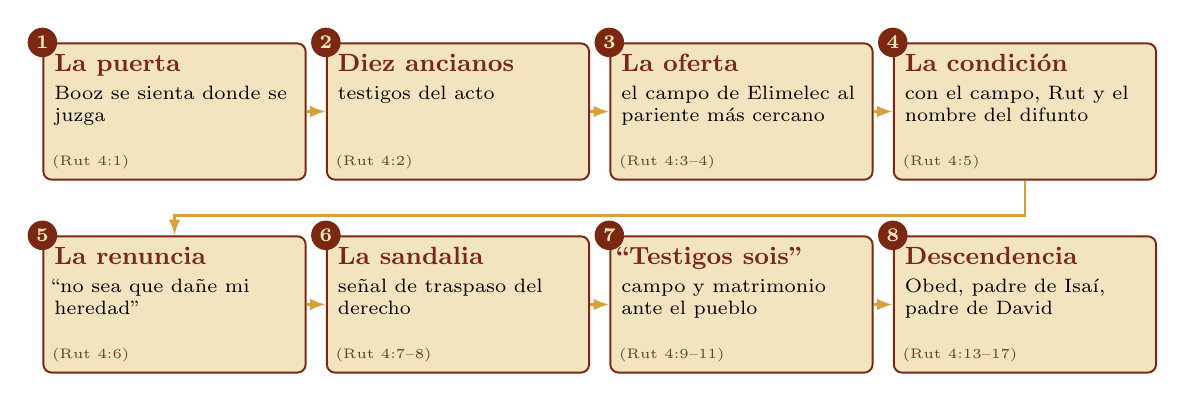
\begin{tikzpicture}[font=\scriptsize]
 \foreach \x/\y/\n/\t/\d/\r in {0/0/1/{La puerta}/{Booz se sienta donde se juzga}/{4:1},
                                 3.6/0/2/{Diez ancianos}/{testigos del acto}/{4:2},
                                 7.2/0/3/{La oferta}/{el campo de Elimelec al pariente más cercano}/{4:3--4},
                                 10.8/0/4/{La condición}/{con el campo, Rut y el nombre del difunto}/{4:5},
                                 0/-2.45/5/{La renuncia}/{``no sea que dañe mi heredad''}/{4:6},
                                 3.6/-2.45/6/{La sandalia}/{señal de traspaso del derecho}/{4:7--8},
                                 7.2/-2.45/7/{``Testigos sois''}/{campo y matrimonio ante el pueblo}/{4:9--11},
                                 10.8/-2.45/8/{Descendencia}/{Obed, padre de Isaí, padre de David}/{4:13--17}}{
  \node[draw=tierraroja,line width=0.7pt,fill=papiro,rounded corners=3pt,anchor=north,inner sep=4pt] (b\n) at (\x,\y) {\parbox[t][1.45cm][t]{3.05cm}{\RaggedRight{\small\textbf{\textcolor{tierraroja}{\t}}}\\[2pt]\scriptsize \d\par\vfill{\tiny\color{sepia}(Rut \r)}}};
  \node[circle,fill=tierraroja,text=papiro,font=\scriptsize\bfseries,inner sep=1.5pt] at (b\n.north west) {\n};}
 \foreach \a/\b in {1/2,2/3,3/4,5/6,6/7,7/8}{\draw[-{Latex[length=2mm]},mostaza,line width=1pt] (b\a.east) -- (b\b.west);}
 \draw[-{Latex[length=2mm]},mostaza,line width=1pt] (b4.south) -- (b4.south |- 0,-2.2) -| (b5.north);
\end{tikzpicture}\par
\pie{\textit{Figura 9.} El rescate en Rut 4: los pasos legales. \textit{Nota.} Elaboración propia con la RVR1960. La relación entre el \emph{goel} de Lv 25 y el levirato de Dt 25 en Rut es discutida (Hubbard, 1988).}
\end{minipage}\end{center}

El pariente anónimo quiere el campo, pero no a Rut: ``No puedo redimir para mí, no sea que dañe mi heredad'' (Rut 4:6). Booz asume las dos cosas. El narrador mide el valor de la redención por su fruto. Las mujeres bendicen a Dios porque ``no te faltase hoy pariente'' (\emph{goel}) y llaman al niño ``restaurador de tu alma'' (Rut 4:14--15); su genealogía termina en David (4:17--22), y el rescate de un campo pasa a formar parte de la historia mesiánica.

\subsection{Jeremías 32: el rescate como esperanza}
Frades Gaspar (1994) observa que Jeremías usa la raíz \emph{g'l} para ``pequeños gestos liberadores, capaces de suscitar y promover la esperanza del pueblo en medio de una situación desesperada''. El más claro es la compra de Anatot. Mientras Babilonia sitia Jerusalén y el profeta está preso en el patio de la cárcel, su primo Hanameel le ofrece el campo familiar, porque a él le corresponde el derecho de herencia y el rescate (Jer 32:7--8). Jeremías lo compra por diecisiete siclos de plata, firma la escritura sellada y la abierta ante testigos y manda guardarlas en una vasija de barro ``para que se conserven muchos días'' (Jer 32:9--14). El sentido del gesto lo da el propio oráculo:

\begin{cita}Porque así ha dicho \SENOR{} de los ejércitos, Dios de Israel: Aún se comprarán casas, heredades y viñas en esta tierra.\fuente{(Jer 32:15)}\end{cita}

La ley del \emph{goel} se vuelve promesa de retorno. El texto no explica la situación de Hanameel ni dice si otros parientes renunciaron antes (Winters, 1994); su interés está en el futuro, y el campo comprado en la ruina es prenda de la tierra restituida.

\subsection{Dios, el \emph{goel} de Israel, en Isaías}
Lo que en la Torá hace el pariente, en Isaías 40--66 lo hace Dios. En mi presentación destaqué que en Isaías 41--63 Dios es llamado ``Redentor'' trece veces (41:14; 43:14; 44:6, 24; 47:4; 48:17; 49:7, 26; 54:5, 8; 59:20; 60:16; 63:16). Un conteo propio sobre el Códice de Leningrado muestra que las trece traducen el mismo participio \emph{goel}, once de ellas con sufijo posesivo (``tu'', ``su'', ``vuestro'', ``nuestro Redentor''); la cifra de nueve que da la fuente no se confirma. Arango (1994) muestra que la identidad del Redentor se define por su relación con el pueblo: Dios lo creó y lo formó, lo salvó de Egipto y vuelve a rescatarlo de Babilonia. Los títulos que acompañan a \emph{goel} lo confirman:

\begin{center}\begin{minipage}{\linewidth}\centering\small\renewcommand{\arraystretch}{1.18}
\begin{tabular}{@{}L{5.2cm}L{6.4cm}L{3.0cm}@{}}
\toprule
\textbf{Título} & \textbf{Texto (RVR1960)} & \textbf{Referencia} \\ \midrule
el Santo de Israel & ``tu Redentor, el Santo de Israel'' & Is 41:14; 47:4; 48:17 \\
Creador y Rey & ``Redentor vuestro\ldots{} Creador de Israel, vuestro Rey'' & Is 43:14--15 \\
\SENOR{} de los ejércitos & ``Rey de Israel, y su Redentor, \SENOR{} de los ejércitos'' & Is 44:6 \\
el Fuerte de Jacob & ``Salvador tuyo y Redentor tuyo, el Fuerte de Jacob'' & Is 49:26; 60:16 \\
el esposo & ``tu marido es tu Hacedor\ldots{} tu Redentor, el Santo de Israel'' & Is 54:5 \\
el Padre & ``tú, oh \SENOR, eres nuestro padre; nuestro Redentor perpetuo'' & Is 63:16 \\
\bottomrule
\end{tabular}\par
\pie{\textit{Tabla 5.} Los títulos del \emph{goel} en Isaías. \textit{Nota.} Elaboración propia a partir de mi presentación anterior \emph{El Jubileo} y de Arango (1994).}
\end{minipage}\end{center}

La redención de Isaías tiene dos referentes históricos. El primero es el éxodo: Dios es ``el que transformó en camino las profundidades del mar para que pasaran los redimidos'' (Is 51:10), y ``en su amor y en su clemencia los redimió'' (Is 63:9). El segundo es Babilonia: ``Salid de Babilonia\ldots{} decid: Redimió \SENOR{} a Jacob su siervo'' (Is 48:20); ``De balde fuisteis vendidos; por tanto, sin dinero seréis rescatados'' (Is 52:3). El rescate es personal, como el del pariente (``No temas, porque yo te redimí; te puse nombre, mío eres tú'', Is 43:1), y su resultado es un pueblo con nombre nuevo: ``Y les llamarán Pueblo Santo, Redimidos de \SENOR'' (Is 62:12); ``los redimidos de \SENOR{} volverán, y vendrán a Sion con alegría'' (Is 35:10). Pablo cita la promesa de Is 59:20, ``vendrá el Redentor a Sion'', para la salvación final de Israel (Ro 11:26).

%===================================================================
\section{El año de la redención}

\subsection{Isaías 63: ``el año de mis redimidos ha llegado''}
En mi presentación dediqué una lámina a Isaías 63:1--6 bajo el título ``el año de la redención''. El poema presenta a un guerrero que viene de Edom, de Bosra, ``con vestidos rojos''; ha pisado solo el lagar de los pueblos (Is 63:1--3). La razón está en el v.~4:

\hebverso{כִּי יוֹם נָקָם בְּלִבִּי וּשְׁנַת גְּאוּלַי בָּאָה}
\begin{cita}Porque el día de la venganza está en mi corazón, y el año de mis redimidos ha llegado.\fuente{(Is 63:4)}\end{cita}

``El año de mis redimidos'' (\heb{שְׁנַת גְּאוּלַי}, \emph{shenat ge'ulay}) usa la raíz del \emph{goel}. El versículo invierte el orden de Is 61:2, donde ``el año de la buena voluntad'' precede al ``día de venganza''; aquí ``el día de la venganza'' precede al ``año de mis redimidos''. Isaías 34:8 ya había formulado el par: ``Porque es día de venganza de \SENOR, año de retribuciones en el pleito de Sion''. El año es largo y es de gracia; el día es breve y es de juicio. En mi presentación de Yom Kipur leí Is 63:4 como el anuncio del Jubileo final: ``el año de mi redención (Jubileo) ha llegado''.

\begin{center}\begin{minipage}{\linewidth}\centering
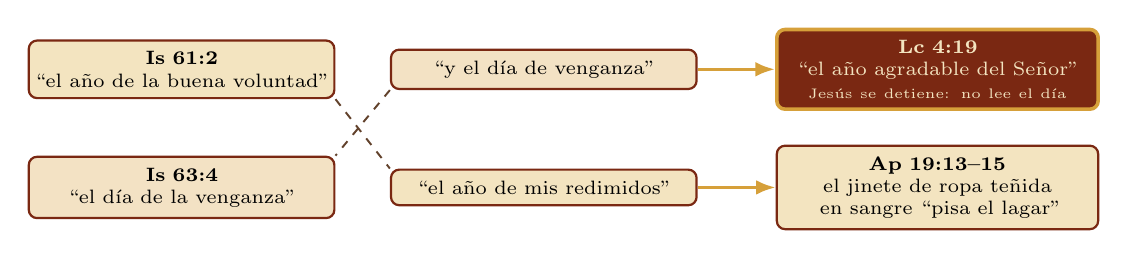
\begin{tikzpicture}[font=\scriptsize]
 \node[draw=tierraroja,line width=0.8pt,fill=papiro,rounded corners=3pt,text width=3.6cm,align=center,inner sep=4pt] (a1) at (0,1.3) {\textbf{Is 61:2}\\ ``el año de la buena voluntad''};
 \node[draw=tierraroja,line width=0.8pt,fill=mostaza!30,rounded corners=3pt,text width=3.6cm,align=center,inner sep=4pt] (a2) at (4.6,1.3) {``y el día de venganza''};
 \node[draw=tierraroja,line width=0.8pt,fill=mostaza!30,rounded corners=3pt,text width=3.6cm,align=center,inner sep=4pt] (b1) at (0,-0.2) {\textbf{Is 63:4}\\ ``el día de la venganza''};
 \node[draw=tierraroja,line width=0.8pt,fill=papiro,rounded corners=3pt,text width=3.6cm,align=center,inner sep=4pt] (b2) at (4.6,-0.2) {``el año de mis redimidos''};
 \draw[sepia,line width=0.7pt,dashed] (a1.south east) -- (b2.north west);
 \draw[sepia,line width=0.7pt,dashed] (a2.south west) -- (b1.north east);
 \node[draw=mostaza,line width=1.3pt,fill=tierraroja,text=papiro,rounded corners=3pt,text width=3.8cm,align=center,inner sep=4pt] (l) at (9.6,1.3) {\textbf{Lc 4:19}\\ ``el año agradable del Señor''\\ {\tiny Jesús se detiene: no lee el día}};
 \node[draw=tierraroja,line width=0.8pt,fill=papiro,rounded corners=3pt,text width=3.8cm,align=center,inner sep=4pt] (r) at (9.6,-0.2) {\textbf{Ap 19:13--15}\\ el jinete de ropa teñida en sangre ``pisa el lagar''};
 \draw[-{Latex[length=2.5mm]},mostaza,line width=1.2pt] (a2.east) -- (l.west);
 \draw[-{Latex[length=2.5mm]},mostaza,line width=1.2pt] (b2.east) -- (r.west);
\end{tikzpicture}\par
\pie{\textit{Figura 10.} El día y el año: Is 61:2 e Is 63:4 en quiasmo, y su lectura en el Nuevo Testamento. \textit{Nota.} Elaboración propia con la RVR1960. La conexión con Ap 19 es un eco de Is 63:1--3 (lagar, vestidos teñidos), no una cita explícita.}
\end{minipage}\end{center}

\subsection{Abdías: ``la casa de Jacob recuperará sus posesiones''}
En esa misma presentación uní Isaías 63 con Abdías, y la conexión tiene base textual, porque los dos pasajes se dirigen contra Edom. Abdías anuncia: ``Porque cercano está el día de \SENOR{} sobre todas las naciones; como tú hiciste se hará contigo'' (Abd 15). Y después del juicio, la restitución:

\hebverso{וּבְהַר צִיּוֹן תִּהְיֶה פְלֵיטָה וְהָיָה קֹדֶשׁ וְיָרְשׁוּ בֵּית יַעֲקֹב אֵת מוֹרָשֵׁיהֶם}
\begin{cita}Mas en el monte de Sion habrá un remanente que se salve; y será santo, y la casa de Jacob recuperará sus posesiones.\fuente{(Abd 17)}\end{cita}

El vocabulario no es el de Levítico 25 (\emph{yarash}, ``poseer, heredar'', y \emph{morashá}, ``posesión'', en lugar de \emph{ajuzá}), pero la idea sí es la del Jubileo: después del día del \SENOR, cada uno vuelve a su heredad. El libro termina con la frase que resume la esperanza, ``y el reino será de \SENOR'' (Abd 21).

\subsection{Del año de gracia al año de los redimidos}
Puestos en secuencia, los textos dibujan un recorrido. Isaías 61:1--3 anuncia al ungido que proclama \emph{derór} y el año de la buena voluntad; Lucas 4:16--21 lo declara cumplido ``hoy'' y se detiene antes del día de venganza; Hechos 3:21 sitúa la ``restauración de todas las cosas'' en el futuro, cuando el cielo deje de retener a Cristo; Isaías 63:4 y Abdías 15--21 describen el día del \SENOR{} y el año de los redimidos, con la recuperación de las posesiones; Ezequiel 46:17 coloca ``el año de la libertad'' en el orden del templo restaurado. En mi presentación concluí que el Mesías es ``nuestro \emph{Goel}'', el que proclamó el año de gracia en su primera venida y traerá el año de sus redimidos en la segunda.

\begin{nota}[Precisión]
Isaías 63:4 no usa la palabra \emph{yovel} ni \emph{derór}: dice ``el año de mis redimidos'' (\emph{ge'ulay}). Su lectura como el Jubileo final es tipológica y depende de la raíz común con la \emph{ge'ulá} de Lv 25:24 y del paralelo con Is 61:2. La distribución entre una primera venida (el año de gracia) y una segunda (el día de venganza) es la lectura cristiana tradicional de Lc 4:19--20, no una afirmación explícita de Lucas.
\end{nota}

%===================================================================
\section{Memorial, figura y esperanza: la lectura de la serie}

\subsection{El marco: Reglamento de Culto, expiación y plan de salvación}
El documento de referencia de la serie lee Levítico 23 como el ``Reglamento del Culto'': las solemnidades del \SENOR, proclamadas convocaciones santas, distintas de la ley de los sacrificios (Lv 1--7; Nm 28--29). Cada fiesta es a la vez \emph{memorial} de un hito de la historia de Israel y \emph{figura} de una etapa del plan de salvación. En ese esquema, las fiestas del otoño forman una secuencia: Trompetas (el retorno de Cristo a la final trompeta), Expiación (el fin del juicio a la casa de Dios y la atadura de Satanás, figurada en el macho cabrío para Azazel), Cabañas (el Reino milenial) y el Octavo día (el tiempo posterior al Milenio y el juicio final), y detrás de todo el sábado, figura del ``reposo'' que queda para el pueblo de Dios (He 4:9; Ap 21:1--4).

El documento no trata el Jubileo, pero el Jubileo encaja en el marco con naturalidad, por tres razones que el propio texto bíblico ofrece:
\begin{enumerate}\setlength{\itemsep}{1pt}
\item \textbf{Se anuncia en una de las convocaciones.} El shofar del Jubileo suena ``el día de la expiación'' (Lv 25:9), dentro del Reglamento de Culto. El año de liberación nace de la solemnidad del perdón.
\item \textbf{Tiene un hito histórico.} El Jubileo presupone la entrada en Canaán y el reparto de las heredades por suerte (Lv 25:2; Jos 13--21). La serie asocia Cabañas con la entrada en la tierra y el establecimiento de Israel como reino; el Jubileo es la ley que protege ese reparto para que cada generación vuelva a él.
\item \textbf{Tiene una esperanza profética.} Isaías 61 lo proyecta a la restauración final, Jesús lo proclama en Nazaret y los apóstoles describen la consumación con su lenguaje: la ``redención de la posesión adquirida'' (Ef 1:14), la creación ``libertada de la esclavitud de corrupción'' (Ro 8:21), ``los tiempos de la restauración de todas las cosas'' (Hch 3:21).
\end{enumerate}

\subsection{Expiación, libertad, retorno}
La lectura de la serie puede formularse así: en el Jubileo, la expiación no termina en el santuario. Una vez quitado el pecado, Dios devuelve a cada uno su libertad, su heredad y su familia. En mi presentación sobre Yom Kipur lo escribí sin matices: ``El año del Jubileo era el Día de Expiación''; Yeshua vino a predicar esa libertad en su primera venida (Is 61:1--3; Lc 4:17--21), y ``el verdadero cumplimiento del año del Jubileo tomará lugar en la segunda venida del Mesías'', cuando la tierra sea redimida de la maldición, el pueblo de Dios quede libre ``de todo pecado, enfermedad, muerte y maldición'', Satanás sea atado y el tabernáculo de Dios esté con los hombres (Ap 21:1--4). El folleto de la Iglesia de Dios Unida lee Is 61:1--3 en el mismo sentido, como la curación que comenzará en el Reino (Iglesia de Dios Unida, 2011).

\begin{center}\begin{minipage}{\linewidth}\centering
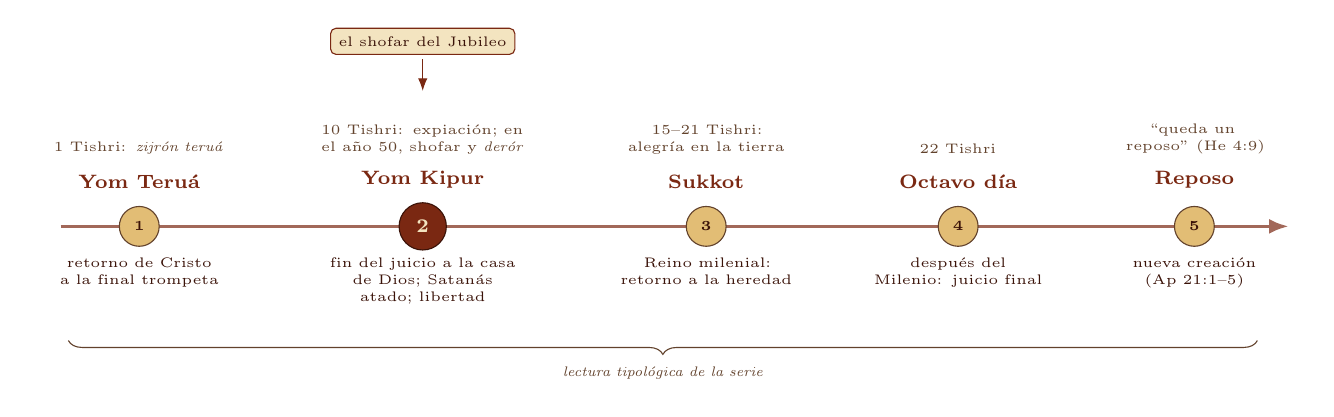
\begin{tikzpicture}[x=1cm,y=1cm,font=\scriptsize]
 \draw[line width=1.3pt,tierraroja!70,-{Latex[length=2.5mm]}] (0,0) -- (15.6,0);
 \foreach \x/\n/\t/\d/\s in {1.0/1/{Yom Teruá}/{1 Tishri: \emph{zijrón teruá}}/{retorno de Cristo a la final trompeta},
                             4.6/2/{Yom Kipur}/{10 Tishri: expiación; en el año 50, shofar y \emph{derór}}/{fin del juicio a la casa de Dios; Satanás atado; libertad},
                             8.2/3/{Sukkot}/{15--21 Tishri: alegría en la tierra}/{Reino milenial: retorno a la heredad},
                             11.4/4/{Octavo día}/{22 Tishri}/{después del Milenio: juicio final},
                             14.4/5/{Reposo}/{``queda un reposo'' (He 4:9)}/{nueva creación (Ap 21:1--5)}}{
   \ifnum\n=2
    \node[circle,fill=tierraroja,draw=caferojizo,minimum size=6mm,text=papiro,font=\scriptsize\bfseries] at (\x,0) {\n};
   \else
    \node[circle,fill=mostaza!70,draw=sepia,minimum size=5mm,text=caferojizo,font=\tiny\bfseries] at (\x,0) {\n};
   \fi
   \node[above=6pt,font=\scriptsize\bfseries,text=tierraroja] at (\x,0.15) {\t};
   \node[above=17pt,font=\tiny,text=sepia,text width=2.6cm,align=center] at (\x,0.2) {\d};
   \node[below=8pt,font=\tiny,text=caferojizo,text width=2.6cm,align=center] at (\x,0) {\s};}
 \draw[decorate,decoration={brace,amplitude=5pt,mirror},sepia] (0.1,-1.45) -- (15.2,-1.45) node[midway,below=6pt,font=\tiny\itshape,text=sepia] {lectura tipológica de la serie};
 \node[draw=tierraroja,fill=papiro,rounded corners=2pt,font=\tiny,align=center,inner sep=3pt,text=caferojizo] at (4.6,2.35) {el shofar del Jubileo};
 \draw[-{Latex[length=1.6mm]},tierraroja] (4.6,2.12) -- (4.6,1.72);
\end{tikzpicture}\par
\pie{\textit{Figura 11.} La secuencia otoñal y el Jubileo: Teruá, Kipur, Sukkot, Octavo día y reposo. \textit{Nota.} Elaboración propia. Arriba, el dato del texto (Lv 23; 25:9); abajo, la lectura de la serie.}
\end{minipage}\end{center}

El shofar une los momentos. Suena en Teruá como memorial (Lv 23:24), suena en el Jubileo para anunciar la liberación (Lv 25:9), y el Nuevo Testamento anuncia una ``final trompeta'' en la resurrección (1~Co 15:52; 1~Ts 4:16). Isaías ya había unido trompeta y retorno: ``Acontecerá también en aquel día, que se tocará con gran trompeta, y vendrán los que habían sido esparcidos en la tierra de Asiria, y los que habían sido desterrados a Egipto, y adorarán a \SENOR{} en el monte santo, en Jerusalén'' (Is 27:13). La trompeta que reúne a los dispersos tiene la forma del Jubileo, en que cada uno vuelve a su tierra.

\begin{nota}[Precisión]
\textbf{1.} El vínculo entre el Jubileo y la segunda venida, el Milenio o la nueva creación es una lectura tipológica, no una afirmación de Levítico. El texto bíblico sí establece que el Jubileo se anuncia en el Día de la Expiación (Lv 25:9) y que Isaías 61 usa su lenguaje para la restauración futura; Lucas 4 lo aplica al ministerio de Jesús.\\
\textbf{2.} El documento de referencia relaciona Trompetas con Jericó y Expiación con el fin del juicio del desierto; esos vínculos son de la serie. Para el Jubileo hay un dato que merece la misma cautela: en Jericó sonaron los \heb{שׁוֹפְרוֹת הַיּוֹבְלִים}, ``las bocinas de \emph{yovel}'' (Jos 6:4--5), al comienzo de la toma de la tierra que el Jubileo protegerá.\\
\textbf{3.} El cálculo de ``casi 6000 años y 120 jubileos'' desde Adán, presente en mi material de Yom Kipur, depende de una cronología bíblica discutida y de leer Gn 6:3 como cifra de la historia; se expone como lectura, no como dato.\\
\textbf{4.} La serie entiende Cabañas como el Milenio y no como la eternidad, porque la cabaña es provisoria. El Jubileo, que devuelve la heredad y comienza un ciclo nuevo, ofrece una imagen complementaria del reposo final: ya no la morada provisoria, sino la herencia restituida (cf. 1~P 1:4, ``una herencia incorruptible, incontaminada e inmarcesible, reservada en los cielos'').
\end{nota}

\subsection{Los tres períodos y el Jubileo}
El documento distingue tres períodos de la Ley y de la Iglesia: la Congregación de los Primogénitos (Adán--Abraham), Israel como congregación del desierto (Hch 7:38) y la Iglesia del Nuevo Pacto. El Jubileo atraviesa los tres. Abraham vivió como \emph{guer ve-toshav} en Hebrón (Gn 23:4) y ``habitó como extranjero en la tierra prometida como en tierra ajena, morando en tiendas'' (He 11:9); recibió la promesa de una \emph{ajuzá} perpetua (Gn 17:8). Israel recibió la tierra y la ley que impedía perderla para siempre (Lv 25:23). La Iglesia recibe ``las arras de nuestra herencia hasta la redención de la posesión adquirida'' (Ef 1:14) y confiesa con los patriarcas que es ``extranjera y peregrina'' (He 11:13; 1~P 2:11). La condición de forastero que fundaba el Jubileo (``vosotros forasteros y extranjeros sois para conmigo'') es la misma que define a la Iglesia mientras espera la heredad.

%===================================================================
\section{El Jubileo en Jesús y los apóstoles}

\subsection{``Hoy se ha cumplido esta Escritura'' (Lc 4:16--30)}
Lucas coloca la escena de Nazaret al comienzo del ministerio público, a modo de programa. Jesús ``vino a Nazaret, donde se había criado; y en el día de reposo entró en la sinagoga, conforme a su costumbre'' (Lc 4:16). Lee Isaías 61 con Isaías 58:6 (véase §5.1), enrolla el libro y se sienta. ``Y los ojos de todos en la sinagoga estaban fijos en él. Y comenzó a decirles: Hoy se ha cumplido esta Escritura delante de vosotros'' (Lc 4:20--21).

\begin{cita}El Espíritu del Señor está sobre mí, Por cuanto me ha ungido para dar buenas nuevas a los pobres; Me ha enviado a sanar a los quebrantados de corazón; A pregonar libertad a los cautivos, Y vista a los ciegos; A poner en libertad a los oprimidos; A predicar el año agradable del Señor.\fuente{(Lc 4:18--19)}\end{cita}

Tres rasgos ligan la escena al Jubileo. El primero es el heraldo: el ungido ``pregona'' (\grc{κηρύξαι}) la \grc{ἄφεσις}, como el Israel de Lv 25:10 proclamaba \emph{derór}. El segundo es el tiempo: ``el año agradable del Señor'' es un año y no un día, y la palabra ``hoy'' (\grc{σήμερον}) lo declara presente. El tercero es el alcance, que se advierte en la reacción de Nazaret cuando Jesús recuerda a la viuda de Sarepta y a Naamán el sirio (Lc 4:25--27), extranjeros beneficiados por Elías y Eliseo. El Jubileo de Jesús rebasa los límites que la letra de Lv 25:44--46 dejaba en pie.

\subsection{La respuesta a Juan (Lc 7:22; Mt 11:5)}
Cuando los discípulos de Juan preguntan si Jesús es ``el que había de venir'', la respuesta enumera hechos que evocan Isaías 35:5--6 y 61:1: ``los ciegos ven, los cojos andan, los leprosos son limpiados, los sordos oyen, los muertos son resucitados, y a los pobres es anunciado el evangelio'' (Lc 7:22). El último miembro (\grc{πτωχοὶ εὐαγγελίζονται}) repite Is 61:1 LXX; las obras de Jesús son el contenido del año agradable.

\subsection{Cristo, el \emph{goel}}
La ley del Jubileo exigía que el rescatador fuera un pariente, y el Nuevo Testamento presenta la encarnación como el cumplimiento de esa condición. Hebreos lo dice expresamente: ``el que santifica y los que son santificados, de uno son todos; por lo cual no se avergüenza de llamarlos hermanos'' (He 2:11); y ``por cuanto los hijos participaron de carne y sangre, él también participó de lo mismo, para destruir por medio de la muerte al que tenía el imperio de la muerte, esto es, al diablo, y librar a todos los que por el temor de la muerte estaban durante toda la vida sujetos a servidumbre'' (He 2:14--15). El hermano que se hace pariente para rescatar al siervo es el \emph{goel} de Lv 25:48--49.

Jesús mismo había definido su misión con el lenguaje del rescate: ``el Hijo del Hombre no vino para ser servido, sino para servir, y para dar su vida en rescate por muchos (Mc 10:45); Mezzacasa (1994) lee el dicho como el resumen de una vida entregada al servicio liberador del \emph{goel}, antes que como una teoría de la satisfacción. Pablo lo expresa con el verbo de la compra: ``Pero cuando vino el cumplimiento del tiempo, Dios envió a su Hijo, nacido de mujer y nacido bajo la ley, para que redimiese (\grc{ἐξαγοράσῃ}) a los que estaban bajo la ley, a fin de que recibiésemos la adopción de hijos'' (Gá 4:4--5). ``Nacido de mujer'' es la condición de parentesco; ``la adopción'', el retorno a la familia. Gálatas 3:13 da el precio: ``Cristo nos redimió de la maldición de la ley, hecho por nosotros maldición''. Tito 2:14 y 1~Pedro 1:18--19 usan \grc{λυτρόω}: ``fuisteis rescatados\ldots{} no con cosas corruptibles, como oro o plata, sino con la sangre preciosa de Cristo, como de un cordero sin mancha y sin contaminación''. Y el cántico de Apocalipsis 5:9 celebra al Cordero porque ``con tu sangre nos has redimido para Dios''.

\begin{center}\begin{minipage}{\linewidth}\centering
\begin{tikzpicture}[font=\scriptsize,node distance=0.55cm]
 \node[draw=tierraroja,line width=0.8pt,fill=papiro,rounded corners=3pt,text width=3.2cm,align=center,inner sep=5pt] (a) {\textbf{El pariente}\\[2pt] rescata campo y persona\\ {\tiny (Lv 25:25, 48--49; Rut 4)}};
 \node[draw=tierraroja,line width=0.8pt,fill=papiro,rounded corners=3pt,text width=3.2cm,align=center,inner sep=5pt,right=of a] (b) {\textbf{Dios, \emph{goel} de Israel}\\[2pt] del éxodo al retorno\\ {\tiny (Éx 6:6; Is 41:14; 43:14; 44:6)}};
 \node[draw=tierraroja,line width=0.8pt,fill=papiro,rounded corners=3pt,text width=3.2cm,align=center,inner sep=5pt,right=of b] (c) {\textbf{``Mi Redentor vive''}\\[2pt] \heb{גֹּאֲלִי חָי}\\ {\tiny (Job 19:25)}};
 \node[draw=mostaza,line width=1.4pt,fill=tierraroja,text=papiro,rounded corners=3pt,text width=3.2cm,align=center,inner sep=5pt,right=of c] (d) {\textbf{Cristo, el hermano}\\[2pt] ``nacido de mujer'', ``participó de lo mismo''\\ {\tiny (Gá 4:4--5; He 2:14--15; Ap 5:9)}};
 \draw[-{Latex[length=3mm]},mostaza,line width=1.3pt] (a)--(b);
 \draw[-{Latex[length=3mm]},mostaza,line width=1.3pt] (b)--(c);
 \draw[-{Latex[length=3mm]},mostaza,line width=1.3pt] (c)--(d);
 \node[below=0.3cm of $(b.south)!0.5!(c.south)$,font=\footnotesize\itshape,text=sepia,text width=13cm,align=center] {El derecho de rescate pertenece al pariente: por eso el Redentor se hace hermano.};
\end{tikzpicture}\par
\pie{\textit{Figura 12.} El \emph{goel} en la Biblia: del pariente a Cristo. \textit{Nota.} Elaboración propia con la BHS y NA28. La lectura cristológica de Job 19:25 es tradicional; en su contexto, Job espera a Dios como su defensor.}
\end{minipage}\end{center}

\begin{nota}[Precisión: autoría de Hebreos]
El documento de referencia atribuye Hebreos a Pablo, como buena parte de la tradición antigua. La autoría es discutida desde la Antigüedad (Orígenes ya dudaba) y la carta es anónima; muchos comentaristas modernos la atribuyen a un autor del círculo paulino (Lane, 1991). El argumento de este apartado no depende de Hebreos, porque Gálatas 4:4--5, una carta paulina indiscutida, expresa la misma idea del Redentor ``nacido de mujer'' que rescata y devuelve a la familia.
\end{nota}

\subsection{La creación liberada (Ro 8:19--23)}
Romanos 8 lleva la lógica del Jubileo hasta la tierra misma: ``porque también la creación misma será libertada de la esclavitud de corrupción, a la libertad gloriosa de los hijos de Dios'' (Ro 8:21). La tierra que en Lv 25 descansaba y volvía a sus dueños gime ahora ``a una, y a una está con dolores de parto hasta ahora'' (v.~22). Los creyentes, que ya tienen ``las primicias del Espíritu'', esperan ``la adopción, la redención de nuestro cuerpo'' (v.~23). Pablo reúne en un versículo tres vocabularios que la serie ha ido recogiendo: las primicias (Shavuot), la adopción (el retorno a la familia) y la redención (la \emph{ge'ulá} del Jubileo).

\subsection{``Los tiempos de la restauración de todas las cosas'' (Hch 3:19--21)}
En el pórtico de Salomón, Pedro llama a Israel: ``arrepentíos y convertíos, para que sean borrados vuestros pecados; para que vengan de la presencia del Señor tiempos de refrigerio, y él envíe a Jesucristo, que os fue antes anunciado; a quien de cierto es necesario que el cielo reciba hasta los tiempos de la restauración de todas las cosas, de que habló Dios por boca de sus santos profetas'' (Hch 3:19--21). La secuencia es la del Jubileo según Levítico: el pecado borrado, el tiempo de alivio y la restauración (\grc{ἀποκατάστασις}) de lo que se había perdido.

\subsection{El reposo final}
Hebreos 4 lee la entrada en Canaán como un reposo incompleto: ``si Josué les hubiera dado el reposo, no hablaría después de otro día. Por tanto, queda un reposo para el pueblo de Dios'' (He 4:8--9). El Jubileo, sábado de los sábados de la tierra, ofrece la figura más amplia de ese reposo, porque en él la tierra descansa, la deuda se cancela y el siervo vuelve a su casa. Apocalipsis 21 lo describe con imágenes de restitución: ``Enjugará Dios toda lágrima de los ojos de ellos; y ya no habrá muerte, ni habrá más llanto, ni clamor, ni dolor''; y el que está sentado en el trono dice: ``He aquí, yo hago nuevas todas las cosas'' (Ap 21:4--5).

%===================================================================
\section{El Jubileo en la tradición judía}

La tradición rabínica trató el Jubileo con detalle, aunque lo consideraba suspendido desde el exilio de las tribus.
\begin{itemize}\setlength{\itemsep}{1pt}
\item \textbf{El shofar del Jubileo.} La Misná equipara el Jubileo a Rosh Hashaná en el toque del shofar y en las bendiciones (m.~\emph{Rosh Hashaná} 3:5), y discute si el shofar del Jubileo es recto o curvo. El Talmud describe los días entre el 1 y el 10 de Tishri del año cincuenta como un tiempo intermedio para los siervos, que salían en Yom Kipur (b.~\emph{Rosh Hashaná} 8b).
\item \textbf{La suspensión.} El Jubileo rige solo cuando ``todos sus moradores'' habitan la tierra; cesó con el exilio de Rubén, Gad y media tribu de Manasés (b.~\emph{Arajin} 32b; \emph{Sifra}, \emph{Behar}). Maimónides lo codifica así en \emph{Hiljot Shemitá ve-Yovel}.
\item \textbf{El \emph{prozbul}.} Cuando la remisión de deudas del año séptimo (Dt 15:1--2) hizo que nadie prestara antes del sabático, Hillel instituyó el \emph{prozbul}, una declaración ante el tribunal que transfería la deuda al tribunal y la preservaba (m.~\emph{Sheviit} 10:3--4). Muestra cómo la tradición adaptó las leyes del ciclo septenario a una economía distinta.
\item \textbf{La práctica actual.} En el Estado de Israel se observa la \emph{shemitá} agrícola con distintas soluciones legales; el Jubileo no se celebra.
\end{itemize}

\begin{nota}[Precisión]
Estas fuentes son de los siglos II--XII e.\,c. y muestran cómo el judaísmo rabínico entendió y aplicó la ley; no describen necesariamente la práctica del Israel bíblico. El \emph{prozbul} y las soluciones modernas para la \emph{shemitá} son desarrollos posteriores.
\end{nota}

%===================================================================
\section{Discusión de interpretaciones}

\subsection{¿Ley histórica o utopía?}
Las posturas quedaron expuestas en §3.3. De Vaux (1985) y Fager (1993) leen el Jubileo como una ley ideal o como un programa posterior al exilio; Milgrom (2001), Bergsma (2007) y Wright (2004) defienden raíces más antiguas y una coherencia con la sociedad de clanes. Ambos grupos coinciden en que el texto se presenta como ley y no como utopía, y en que los profetas lo trataron como norma incumplida (Jer 34; Is 5:8; Ez 46).

\subsection{¿Programa social o anuncio espiritual?}
El debate más vivo gira en torno a Lucas 4.
\begin{itemize}\setlength{\itemsep}{1pt}
\item \textbf{Un Jubileo social.} Yoder (1972), siguiendo a André Trocmé, sostuvo que Jesús proclamó un Jubileo real, con consecuencias económicas (perdón de deudas, redistribución), y que el Padrenuestro (``perdónanos nuestras deudas'', Mt 6:12) conserva ese sentido. Ringe (1985) mostró cómo las imágenes del Jubileo (liberación, perdón, banquete) atraviesan Lucas y piden una ética de la liberación. Sloan (1977) estudió la ``teología jubilar'' de Lucas.
\item \textbf{Un anuncio escatológico y espiritual.} Otros comentaristas aceptan el trasfondo jubilar, pero subrayan que Lucas no menciona el Jubileo por nombre, que no hay indicios de que Jesús convocara a devolver tierras, y que la \grc{ἄφεσις} de Lucas es sobre todo perdón de pecados (Fitzmyer, 1981; Bock, 1994).
\item \textbf{Una lectura integral.} Wright (2004) propone leer el Jubileo en tres niveles: paradigmático (un modelo ético para la economía y la deuda), tipológico (cumplido en la redención de Cristo) y escatológico (la restauración de todas las cosas). Así evita reducir el texto a un programa político y también espiritualizarlo hasta borrar su contenido social.
\end{itemize}
La campaña ``Jubileo 2000'', que pidió la cancelación de la deuda externa de los países más pobres, mostró la vigencia pública del tema.

\subsection{La lectura de la serie entre las demás}
La lectura de la serie (el Jubileo como figura de la redención completa y del Reino) se ubica cerca de la lectura escatológica y tipológica, pero comparte con la lectura social una convicción: la redención que Dios promete no es solo interior, sino que incluye un cuerpo redimido (Ro 8:23), una tierra liberada (Ro 8:21) y una herencia restituida (Ef 1:14; 1~P 1:4). Lo que la serie añade es la secuencia del calendario: lo que Yom Kipur hace en el santuario, el Jubileo lo hace en la tierra.

%===================================================================
\section{Síntesis}

\begin{tcolorbox}[enhanced,unbreakable,colback=papiro,colframe=tierraroja,boxrule=1pt,arc=3pt,title={El Jubileo},fonttitle=\bfseries,coltitle=papiro,colbacktitle=tierraroja]
El Jubileo (\heb{יוֹבֵל}) es el año cincuenta, que sigue a siete ciclos sabáticos y se anuncia con el shofar el 10 de Tishri, Día de la Expiación (Lv 25:8--9). En él se proclama \emph{derór} a todos los moradores de la tierra: cada uno vuelve a su posesión y a su familia, la tierra descansa y el hermano vendido sale libre (Lv 25:10--13, 39--41). Su fundamento es que la tierra y el pueblo pertenecen a Dios (Lv 25:23, 42). Los profetas lo hicieron imagen de la restauración (Is 61:1--3; Ez 46:17); Jesús lo proclamó cumplido ``hoy'' (Lc 4:21); los apóstoles describen a Cristo como el pariente que rescata (Gá 4:4--5; He 2:14--15) y esperan la redención de la posesión adquirida (Ef 1:14). En la lectura de la serie es figura de la redención completa: expiación, libertad y retorno a la heredad, hasta el reposo que queda para el pueblo de Dios (He 4:9).
\end{tcolorbox}

\begin{center}\begin{minipage}{\linewidth}\centering\small\renewcommand{\arraystretch}{1.2}
\begin{tabular}{@{}L{3.0cm}L{11.6cm}@{}}
\toprule
\textbf{Lectura} & \textbf{Aporte} \\ \midrule
Histórica & El Jubileo protege el reparto de la tierra por clanes; comparte con los edictos mesopotámicos la idea de remisión (\emph{andurārum}), pero la vuelve periódica, divina y familiar. Su práctica no está atestiguada; su relectura escatológica sí (Jubileos, 11QMelquisedec). \\
Filológica & \emph{Yovel} es el cuerno; \emph{derór}, la liberación; \emph{goel}, el pariente que rescata. La LXX traduce con \grc{ἄφεσις}, la palabra del perdón de pecados en el NT. \\
Textual & Lc 4:18--19 combina Is 61:1--2 LXX con Is 58:6 y se detiene antes del ``día de venganza''; el año cincuenta empieza a regir el Día de la Expiación. \\
Literaria & La cuenta 7\,×\,7\,+\,1 es la de Shavuot; Lv 25 avanza en círculos de redención (tierra, casas, personas) y cierra con el éxodo; Rut 4 y Jer 32 narran al \emph{goel}. \\
Serie & El Jubileo nace de la Expiación: perdón, libertad y retorno a la heredad, figura del Reino y del reposo final (lectura tipológica). \\
Nuevo Testamento & Cristo, ungido heraldo y pariente redentor; la creación y el cuerpo esperan la \grc{ἀπολύτρωσις}; Pedro anuncia la \grc{ἀποκατάστασις} de todas las cosas. \\
\bottomrule
\end{tabular}\par
\pie{\textit{Tabla 6.} Lo que aporta cada lectura. \textit{Nota.} Elaboración propia.}
\end{minipage}\end{center}

%===================================================================
\section{Para la reflexión}
\begin{enumerate}\setlength{\itemsep}{2pt}
\item ``La tierra mía es; pues vosotros forasteros y extranjeros sois para conmigo'' (Lv 25:23). ¿Qué cambia en la manera de tener, comprar o vender cuando se acepta que uno es residente y no dueño absoluto?
\item La ley prohíbe engañar en el precio y cobrar interés al hermano empobrecido, y su única sanción explícita es ``temed a vuestro Dios'' (vv.~17, 36, 43). ¿En qué negocios, préstamos o contratos de la vida diaria ese temor es la única garantía del otro?
\item Booz aceptó lo que el otro pariente rechazó porque ``dañaba su heredad'' (Rut 4:6). ¿Qué costo personal implica redimir a alguien, y qué enseña eso sobre el costo de la redención en Cristo (1~P 1:18--19)?
\item Jeremías compró un campo cuando la ciudad estaba a punto de caer (Jer 32). ¿Qué gestos concretos de esperanza puede hacer hoy quien cree que ``aún se comprarán casas, heredades y viñas''?
\item Jesús dijo ``hoy'' en Nazaret, y Pablo dice ``ahora'' en 2~Corintios 6:2. ¿Qué significa vivir en el año agradable del Señor mientras se espera la redención del cuerpo (Ro 8:23)?
\item La congregación de Nazaret se enojó cuando la liberación alcanzó a una viuda de Sidón y a un sirio (Lc 4:25--29). ¿A quién dejaríamos fuera del Jubileo?
\end{enumerate}

%===================================================================
\section*{Glosario}
\begin{description}\setlength{\itemsep}{2pt}
\item[\emph{Ajuzá}] (\heb{אֲחֻזָּה}). ``Posesión'', lo que uno tiene asido; palabra clave de Lv 25 (vv.~10, 13, 41).
\item[\emph{Andurārum}] (acadio). ``Liberación'' de deudas y esclavos en los edictos reales mesopotámicos; cognado de \emph{derór}.
\item[\emph{Áphesis}] (\grc{ἄφεσις}). ``Remisión, liberación''; en la LXX, el Jubileo (Lv 25:10); en el NT, el perdón de pecados y la libertad de Lc 4:18.
\item[\emph{Apokatástasis}] (\grc{ἀποκατάστασις}). ``Restauración'': ``los tiempos de la restauración de todas las cosas'' (Hch 3:21).
\item[\emph{Apolytrōsis}] (\grc{ἀπολύτρωσις}). ``Redención'' completa (Ro 8:23; Ef 1:7, 14).
\item[\emph{Dektós}] (\grc{δεκτός}). ``Aceptable, agradable'': ``el año agradable del Señor'' (Lc 4:19).
\item[\emph{Derór}] (\heb{דְּרוֹר}). ``Liberación'' proclamada públicamente (Lv 25:10; Is 61:1; Jer 34:8; Ez 46:17).
\item[\emph{Ge'ulá}] (\heb{גְּאֻלָּה}). ``Rescate'': derecho y precio de recuperar lo vendido (Lv 25:24; Rut 4:6).
\item[\emph{Goel}] (\heb{גֹּאֵל}). Pariente redentor; también vengador de la sangre (Nm 35:19) y título de Dios (Is 44:6; Job 19:25).
\item[\emph{Guer ve-toshav}] (\heb{גֵּר וְתוֹשָׁב}). ``Forastero y residente'': la condición de Israel ante Dios (Lv 25:23).
\item[\emph{Mīšarum}] (acadio). ``Justicia, rectitud'': edicto real de remisión de deudas (Ammi-ṣaduqa).
\item[\emph{Najalá}] (\heb{נַחֲלָה}). ``Heredad'' asignada por suerte, que no debe salir de la familia (1~R 21:3; Nm 36:4).
\item[\emph{Prozbul}] (\heb{פְּרוֹזְבּוּל}). Institución de Hillel que preservaba las deudas ante el año sabático (m.~\emph{Sheviit} 10:3).
\item[\emph{Shemitá}] (\heb{שְׁמִטָּה}). ``Remisión'': el año séptimo de descanso de la tierra y de remisión de deudas (Dt 15:1--2).
\item[\emph{Shenat ratsón}] (\heb{שְׁנַת רָצוֹן}). ``Año de la buena voluntad'' (Is 61:2); LXX \grc{ἐνιαυτὸς δεκτός}.
\item[\emph{Tsemitut}] (\heb{צְמִתֻת}). ``Perpetuidad'': venta definitiva, prohibida para la tierra (Lv 25:23, 30).
\item[\emph{Yovel}] (\heb{יוֹבֵל}). ``Cuerno de carnero''; por extensión, el año cincuenta anunciado con él (Lv 25:10; Jos 6:5).
\end{description}

%===================================================================
\section*{Referencias}\markboth{Referencias}{}
\refapa{Arango L., J.~R. (1994). Dios solidario con su pueblo: el go'el en Deuteroisaías. \emph{Revista de Interpretación Bíblica Latinoamericana}, (18), 55--63.}
\refapa{Bauer, W., Danker, F.~W., Arndt, W.~F., \& Gingrich, F.~W. (2000). \emph{A Greek-English lexicon of the New Testament and other early Christian literature} (3.ª ed.). University of Chicago Press. [BDAG]}
\refapa{Bergsma, J.~S. (2007). \emph{The Jubilee from Leviticus to Qumran: A history of interpretation}. Brill.}
\refapa{Bock, D.~L. (1994). \emph{Luke 1:1--9:50} (BECNT). Baker.}
\refapa{Brown, F., Driver, S.~R., \& Briggs, C.~A. (1906). \emph{A Hebrew and English lexicon of the Old Testament}. Clarendon Press.}
\refapa{Danby, H. (Trad.). (1933). \emph{The Mishnah}. Oxford University Press.}
\refapa{De Vaux, R. (1985). \emph{Instituciones del Antiguo Testamento} (A. Ros, Trad.). Herder.}
\refapa{Elliger, K., \& Rudolph, W. (Eds.). (1997). \emph{Biblia Hebraica Stuttgartensia} (5.ª ed.). Deutsche Bibelgesellschaft.}
\refapa{Fager, J.~A. (1993). \emph{Land tenure and the biblical Jubilee: Uncovering Hebrew ethics through the sociology of knowledge}. JSOT Press.}
\refapa{Filón de Alejandría. (1937). \emph{De specialibus legibus} (F.~H. Colson, Trad.; Loeb Classical Library, vol. 7). Harvard University Press.}
\refapa{Fitzmyer, J.~A. (1981). \emph{The Gospel according to Luke I--IX} (AB 28). Doubleday.}
\refapa{Frades Gaspar, E. (1994). El uso de g'l en los profetas preexílicos. \emph{Revista de Interpretación Bíblica Latinoamericana}, (18), 43--53.}
\refapa{García Martínez, F. (1992). \emph{Textos de Qumrán}. Trotta.}
\refapa{Hartley, J.~E. (1992). \emph{Leviticus} (WBC 4). Word Books.}
\refapa{Hoenig, S.~B. (1969). Sabbatical years and the year of Jubilee. \emph{The Jewish Quarterly Review, 59}(3), 222--236.}
\refapa{Hubbard, R.~L. (1988). \emph{The book of Ruth} (NICOT). Eerdmans.}
\refapa{Iglesia de Dios Unida. (2011). \emph{Las fiestas santas de Dios: esperanza segura para toda la humanidad}. Iglesia de Dios Unida.}
\refapa{Josefo, F. (1997). \emph{Antigüedades judías} (J. Vara Donado, Trad.). Akal.}
\refapa{Kobelski, P.~J. (1981). \emph{Melchizedek and Melchireša`} (CBQMS 10). Catholic Biblical Association of America.}
\refapa{Koehler, L., \& Baumgartner, W. (2001). \emph{The Hebrew and Aramaic lexicon of the Old Testament}. Brill. [HALOT]}
\refapa{Lane, W.~L. (1991). \emph{Hebrews 1--8} (WBC 47A). Word Books.}
\refapa{Lemche, N.~P. (1979). Andurārum and mīšarum: Comments on the problem of social edicts and their application in the ancient Near East. \emph{Journal of Near Eastern Studies, 38}(1), 11--22.}
\refapa{López, R. (1994). Redención de la tierra y del pueblo. \emph{Revista de Interpretación Bíblica Latinoamericana}, (18), 31--41.}
\refapa{Lundbom, J.~R. (2004). \emph{Jeremiah 21--36} (AB 21B). Doubleday.}
\refapa{Mezzacasa, F. (1994). Jesús, el go'el. \emph{Revista de Interpretación Bíblica Latinoamericana}, (18), 65--85.}
\refapa{Milgrom, J. (2001). \emph{Leviticus 23--27} (AB 3B). Doubleday.}
\refapa{Nash, G.~B. (2010). \emph{The Liberty Bell}. Yale University Press.}
\refapa{Nestle, E., \& Aland, K. (Eds.). (2012). \emph{Novum Testamentum Graece} (28.ª ed.). Deutsche Bibelgesellschaft.}
\refapa{Nolland, J. (1989). \emph{Luke 1--9:20} (WBC 35A). Word Books.}
\refapa{Rahlfs, A., \& Hanhart, R. (Eds.). (2006). \emph{Septuaginta} (ed. rev.). Deutsche Bibelgesellschaft.}
\refapa{Rashi. (s.f.). \emph{Comentario a la Torá} [Éx 21:6]. Sefaria. https://www.sefaria.org}
\refapa{Ringe, S.~H. (1985). \emph{Jesus, liberation, and the biblical Jubilee: Images for ethics and christology}. Fortress Press.}
\refapa{\emph{Santa Biblia: Reina-Valera 1960}. (1960). Sociedades Bíblicas en América Latina.}
\refapa{Sloan, R.~B. (1977). \emph{The favorable year of the Lord: A study of jubilary theology in the Gospel of Luke}. Schola Press.}
\refapa{Steinsaltz, A. (Ed.). (2017). \emph{Koren Talmud Bavli} [Rosh Hashaná 8b; Arajin 12a, 32b; Nedarim 61a]. Sefaria. https://www.sefaria.org}
\refapa{VanderKam, J.~C. (1998). \emph{Calendars in the Dead Sea Scrolls: Measuring time}. Routledge.}
\refapa{VanderKam, J.~C. (2001). \emph{The Book of Jubilees}. Sheffield Academic Press.}
\refapa{Vermes, G. (2004). \emph{The complete Dead Sea Scrolls in English} (ed. rev.). Penguin.}
\refapa{Weinfeld, M. (1995). \emph{Social justice in ancient Israel and in the ancient Near East}. Fortress Press; Magnes Press.}
\refapa{Wenham, G.~J. (1979). \emph{The book of Leviticus} (NICOT). Eerdmans.}
\refapa{Wight, F.~H. (1953). \emph{Usos y costumbres de las tierras bíblicas}. Portavoz.}
\refapa{Winters, A. (1994). El goel en el antiguo Israel. \emph{Revista de Interpretación Bíblica Latinoamericana}, (18), 19--29.}
\refapa{Wright, C.~J.~H. (2004). \emph{Old Testament ethics for the people of God}. InterVarsity Press.}
\refapa{Yoder, J.~H. (1972). \emph{The politics of Jesus}. Eerdmans.}

\end{document}
